% Options for packages loaded elsewhere

\PassOptionsToPackage{hyphens}{url}
\PassOptionsToPackage{dvipsnames,svgnames*,x11names*}{xcolor}
%
\documentclass[12pt, a4paper]{article}

% Set up fonts

\usepackage{amssymb,amsmath} % Need to load before unicode-math


% Customize floats: always put captions at the top and use the
% afore-defined typeface in tables. This packages also provides the
% `\floatfoot' environment for notes in floats.
\usepackage{floatrow}
\floatsetup[table]{capposition=top, font={small}} % neet this for table caption to go on top
% Make float numbers and labels stand out
\usepackage[labelfont=bf]{caption}

% appendix titles
\usepackage[title]{appendix}

\usepackage[]{microtype}
\UseMicrotypeSet[protrusion]{basicmath} % disable protrusion for tt fonts
\usepackage{xcolor}
\usepackage{xurl} % add URL line breaks
\usepackage{bookmark}
\hypersetup{
  pdftitle={Intersectional Inequality in Education},
  pdfauthor={Dario Meili, Isabel Günther, Kenneth Harttgen},
  pdfkeywords={Inequality, Intersectionality, Measurement, Poverty},
  colorlinks=true,
  linkcolor=Maroon,
  filecolor=Maroon,
  citecolor=Blue,
  urlcolor=Blue,
  pdfcreator={LaTeX via pandoc}}
\urlstyle{same} % disable monospaced font for URLs
\usepackage{geometry}
\geometry{a4paper,
 left=25mm,
 top=25mm}
\usepackage{longtable,booktabs,dcolumn}

\usepackage{calc} % for calculating minipage widths
% Correct order of tables after \paragraph or \subparagraph
\usepackage{etoolbox}
\makeatletter
\patchcmd\longtable{\par}{\if@noskipsec\mbox{}\fi\par}{}{}
\makeatother
% Allow footnotes in longtable head/foot
\usepackage{footnotehyper}
\makesavenoteenv{longtable}
\usepackage{graphicx,subcaption}
\makeatletter
\def\maxwidth{\ifdim\Gin@nat@width>\linewidth\linewidth\else\Gin@nat@width\fi}
\def\maxheight{\ifdim\Gin@nat@height>\textheight\textheight\else\Gin@nat@height\fi}
\makeatother
% Scale images if necessary so that they will not overflow the page
% margins by default, and it is still possible to overwrite the defaults
% using explicit options in \includegraphics[width, height, ...]{}
\setkeys{Gin}{width=\maxwidth,height=\maxheight,keepaspectratio}
\setlength{\emergencystretch}{3em} % prevent overfull lines
\providecommand{\tightlist}{%
  \setlength{\itemsep}{0pt}\setlength{\parskip}{0pt}}
\setcounter{secnumdepth}{3}
\usepackage{float}
\usepackage{placeins}
\usepackage{array}
\usepackage{multirow}
\usepackage{wrapfig}
\usepackage{colortbl}
\usepackage{pdflscape}
\usepackage{tabu}
\usepackage{threeparttable}
\usepackage{threeparttablex}
\usepackage[normalem]{ulem}
%degree symbol
\usepackage{gensymb}
\usepackage{makecell}
\usepackage{siunitx} 
% needed for modelsummary
\usepackage{comment} % needed for commenting out sections
%bibliography
\usepackage{natbib}
\usepackage{setspace}%needed for onehlafspacing
\newcolumntype{d}{S[input-symbols = ()]} 
%needed for modelsummary



\newlength{\cslhangindent}
\setlength{\cslhangindent}{1.5em}
\newlength{\csllabelwidth}
\setlength{\csllabelwidth}{3em}
\newenvironment{CSLReferences}[2] % #1 hanging-ident, #2 entry spacing
 {% don't indent paragraphs
  \setlength{\parindent}{0pt}
  % turn on hanging indent if param 1 is 1
  \ifodd #1 \everypar{\setlength{\hangindent}{\cslhangindent}}\ignorespaces\fi
  % set entry spacing
  \ifnum #2 > 0
  \setlength{\parskip}{#2\baselineskip}
  \fi
 }%
 {}
 
\usepackage{calc}
\newcommand{\CSLBlock}[1]{#1\hfill\break}
\newcommand{\CSLLeftMargin}[1]{\parbox[t]{\csllabelwidth}{#1}}
\newcommand{\CSLRightInline}[1]{\parbox[t]{\linewidth - \csllabelwidth}{#1}\break}
\newcommand{\CSLIndent}[1]{\hspace{\cslhangindent}#1}

\usepackage{quotes}

%make it possible to control margins of landscape tables 
\makeatletter

\def\vfudge#1#2{%
\addtolength\textheight{#1}%
\@colroom\textheight
\vsize\textheight
\@colht\textheight
\def\LS@rot{%
  \setbox\@outputbox\vbox{\hbox{\kern-#2\rotatebox{90}{\box\@outputbox}}}}%
\clearpage}

\makeatother

% tabular array: for tinytable
\usepackage{tabularray}
\usepackage{float}
\usepackage{graphicx}
\usepackage{rotating}
\usepackage[normalem]{ulem}
\UseTblrLibrary{booktabs}
\UseTblrLibrary{siunitx}
\newcommand{\tinytableTabularrayUnderline}[1]{\underline{#1}}
\newcommand{\tinytableTabularrayStrikeout}[1]{\sout{#1}}
\NewTableCommand{\tinytableDefineColor}[3]{\definecolor{#1}{#2}{#3}}

\title{Intersectional Inequality in Education in Africa, Asia, and the Americas}
\author{
   Dario Meili\thanks{Development Economics Group, ETH Zurich, Switzerland, \href{mailto:dario.meili@nadel.ethz.ch}{\nolinkurl{dario.meili@nadel.ethz.ch}} 
  } \and
  Kenneth Harttgen\thanks{
    Development Economics Group, ETH Zürich, Switzerland
  } \and
  Isabel Günther\thanks{
    Development Economics Group, ETH Zürich, Switzerland
    \newline
   The authors thank Dominik Hangartner, Ellora Derenoncourt, participants and discussants at the ETH4D Seminar 2021, the UZH-ETH Development Economics Colloquium 2021, the IARIW, Bridges and VfS Development Conferences 2022, the ECINEQ Conference 2023, and the ETH DEC Group for thoughtful suggestions and comments. In addition, we thank Samuel Tetteh-Baah for his previous work. Thanks are also due to two anonymous referees and Conchita D'Ambrosio, the corresponding editor. This work was supported by an ETH Zurich Doc.Mobility Fellowship. 
  }
}
\date{\today}

\begin{document}
% Create a fake title page because no reasonably long abstract will
% leave enough space at the bottom. And narrow the bottom margin to
% slide footnotes down. See Section 6.4 of the `geometry' package how
% they calculate the default 5.346cm.
\newgeometry{bottom=3cm}
\maketitle
\thispagestyle{empty} % Need to put after \maketitle

%%%%%%%%%%%%%%%%%%%%%%%%%%%%%%%%%%%%%%%
% ABSTRACT
%%%%%%%%%%%%%%%%%%%%%%%%%%%%%%%%%%%%%%%
\begin{abstract}
  \noindent Intersectional inequality --- the notion that disparities run along combinations of social groups such as gender or ethnicity --- has become an increasingly prominent concept in the social sciences. However, there is little empirical research applying an intersectional framework to measure inequality. We propose two novel metrics of intersectional inequality based on the concept of horizontal inequality. Based on these measures, we analyze educational intersectionality in gender and ethnicity using Demographic and Health Survey data from 39 low- and middle-income countries and census data from the United States. We show that the intersectional perspective unveils substantial inequality that remains masked if gender and ethnicity are analyzed in isolation. For countries with high intersectional inequality, which is more than the sum of gender and ethnic inequality, reducing inequalities based on gender and ethnicity separately might not be enough to "leave no one behind," as the 2030 United Nations Agenda envisions.  \\
  
  \noindent \textbf{JEL codes}: D63, I24, J16  \\
    
  \noindent \textbf{Keywords}: Inequality, Intersectionality, Measurement, Education 
  \end{abstract}
\restoregeometry

\onehalfspacing
%%%%%%%%%%%%%%%%%%%%%%%%%%%%%%%%%%%%%%%
% INTRODUCTION
%%%%%%%%%%%%%%%%%%%%%%%%%%%%%%%%%%%%%%%
\hypertarget{introduction}{%
\section{Introduction}\label{introduction}}

\textit{Leave no one behind}, the central principle of the 2030 Agenda for Sustainable Development, highlights that "barriers people face in accessing services, resources and equal opportunities are not simply accidents of fate or a lack of availability of resources, but rather the result of discriminatory laws, policies and social practices that leave particular groups of people further and further behind" \citep{UNSDG2022}. In other words, disadvantages occur not only for individuals but also for whole social groups, for instance, women or members of marginalized ethnic groups. Since individuals have little (or no) influence over group membership, like gender or ethnicity, these systematic disparities are not only problematic from the perspective of equality of opportunity, but they are detrimental to economic development on a broader scale \citep{Ferreira2018, Marrero2013}. In response, economists increasingly apply the concept of horizontal inequality when measuring inequalities between social groups, such as gender or ethnicity \citep{Mancini2008}. 

At the same time, "intersectionality" has become a buzzword in the social sciences. For example, the UN Sustainable Development Group states that identifying inequalities requires disaggregation beyond gender, geography, and age and should occur in multiple and intersecting ways \citep{UNSDG2022}. The term \textit{intersectionality} was coined by \cite{crenshaw1989, Crenshaw1991} as a critical theoretical framework to describe the distinct discrimination faced by members at the "intersection" of social groups. For example, Black women might face specific disadvantages that neither Black men nor white women experience. Similarly, \cite{kabeer2016} uses the term "intersecting inequalities" to highlight individuals' overlapping disadvantages, reinforcing their exclusion. The particular overlaps that characterize marginalization vary by context, but \cite{kabeer2016} points out that the most enduring forms of group-based disadvantages are strongly associated with identities (arguably) ascribed at birth, such as race, caste, gender, and ethnicity. Therefore, this framework could be viewed as an extension of the horizontal inequalities framework. However, intersectionality remains mostly exclusive to theory in the humanities and is only starting to gain traction in the quantitative social sciences. More specifically, there are very few examples directly linking the concept of intersectionality to the measurement of group-based inequalities in low- and middle-income countries \citep[see e.g.,][]{Kabeer2017, Lenhardt2015}.

To fill this gap, our work seeks to reconcile the intersectionality framework with the measurement of horizontal inequalities. In particular, we document and analyze intersectional inequalities in educational attainment in 40 countries by combining gender and ethnicity to form intersecting groups. As long as educational outcomes differ systematically and substantially between social groups, it is unlikely that the world will succeed in 'leaving no one behind', as stated by Agenda 2030 and its Sustainable Development Goals (SDGs) \citep{Stuart2016}. This paper contributes to an analytic framework to detect intersecting group-based inequalities to inform policy-making. Moreover, we also focus on education for analytical reasons, since many other well-being indicators, such as income or wealth, are hardly separable among members of the same household. Thus, measuring gender inequalities in these outcomes is not feasible. Meanwhile, education is an outcome that accrues entirely to the individual, allowing us to analyze gender differences in schooling. 

We descriptively analyze how educational attainment varies across intersecting groups and time. To this end, we combine data from several rounds of the Demographic and Health Surveys (DHS) in 39 low- and middle-income countries between 1992 and 2019, as well as data from the US Current Population Survey (CPS) 2019, resulting in 2,689,289 individual observations. Little is known about intersecting inequalities in the global context and the DHS data pose a unique opportunity to analyze this topic. We include US data since the intersectionality literature has its origins in the US, making it relevant to put the magnitude of the results for low- and middle-income countries into perspective. 

Our first measure of intersectional inequality is the schooling ratio between the group with the lowest (most disadvantaged) and the group with the highest (most advantaged) average education. We do this across gender, ethnicity, and the combination thereof. Compared to other inequality measures, this approach emphasizes the extremes of the distribution, in line with the principle to "leave no one behind." We find that intersectional inequality between ethnicity and gender differs significantly across countries and is larger than horizontal inequality by ethnicity and gender separately. Intersectional inequality is mainly driven by ethnic inequality and less by gender inequality since ethnic inequalities still tend to be more pronounced in many countries. The second measure of intersectionality we propose --- which we refer to as differential intersectionality --- aims to quantify the intersectionality that is "more than the sum of its parts" of gender and ethnic inequality. To this end, we first estimate how much inequality would arise if gender inequality were constant across all ethnic groups as a synthetic counterfactual. We compare this measure with the total, first-order intersectional inequality and calculate the difference, yielding the differential intersectionality measure. In 27 countries, the intersecting inequality is positive, implying that it is greater than what would be expected if all ethnic groups experienced the same gender inequality, and thus "more than the sum of its parts". Interestingly, for 13 countries in the sample, differential intersectionality is negative, indicating less gender inequality in the most advantaged/disadvantaged ethnic groups. 

We use regression analysis to identify the main correlates of horizontal and intersectional inequality. The analysis shows that intersectional inequality in education is not associated with the general level of education when also taking overall inequality in education into account. Countries with higher education Gini tend to have higher intersectional inequality. The number of ethnic groups in a country is also associated with higher intersectional inequality. However, neither mean education, overall education inequality, nor the number of ethnic groups are significantly associated with differential intersectionality. 

The remainder of this paper proceeds as follows. Section~\ref{sec:literature} discusses the related literature. Section~\ref{measures} introduces the concept of intersectional inequalities and describes the empirical strategy to estimate intersectional inequalities and the subsequent analysis. Section~\ref{data} presents more information on the data. Section~\ref{results} presents the results of the analysis. Section~\ref{conclusion} concludes.

\section{Related Literature}\label{sec:literature}

This paper contributes to five different strands of literature touching on intersectional inequality. 

First, on a broader level, this paper speaks to established theoretical literature in sociology, social psychology, and gender studies that conceptualizes intersectionality theoretically. Kimberlé \cite{crenshaw1989} coined the term, and what has followed is an ample discussion about the consequences of adopting an intersectional perspective, not only for social sciences but also for public policy \citep[to name just a few examples:][]{alexander-floyd2012, berger2010, bowleg2008, cho2013, choo2010, few-demo2014, hancock2007, shields2008, strid2013, walby2012}. However, the cited works make little to no prescriptions of \textit{how} intersectionality could be operationalized quantitatively. The paper at hand contributes to this literature by proposing a framework for how researchers could include intersectionality in the quantitative measurement of inequality.

Second, the research that empirically applies an intersectional perspective primarily addresses education inequality at the intersection of race and gender in the US context. A number of studies examine the Black gender gap in college success \citep{Keels2013, McDaniel2011, Mittleman2021}, labor market returns to math performance \citep{Riegle-Crumb2006}, or success expectations in STEM-related subjects \citep[][review article]{Parker2020}. Together, the studies paint a clear picture of intersectional disparities in education. Black women do not fully profit from the generally closing gender gap in education, yet Black men are typically even worse off than Black women. These effects are partly offset by socioeconomic status, especially for black women, implying that there is no gender gap for Black women with high socioeconomic status \citep{Keels2013}. These findings highlight the importance of intersectionality as an analytical framework because they provide essential insights usually lost when considering social identities like race and gender in isolation. However, the methodological frameworks applied in the cited studies are not necessarily applicable to other countries where the concepts of race and ethnic groups differ substantially from the US context.

For example, in the non-US context, \cite{Sen2009} analyze inequality in access to health services at the intersection of gender and social class in India. They find that the probability of non-treatment is only lower for women from poor households while being poor (or "lower class") is not relevant for men. The authors model intersectionality as interaction terms in their regressions and report the probability (odds ratio) of having a particular health-related outcome for members of a social group compared to a reference group. Our study departs from this literature in several aspects. On the one hand, we explicitly relate our empirical analysis to the theoretical literature on intersectionality. As such, intersectionality is not merely meant as an afterthought, but as an analytical lens through which to study inequalities. On the other hand, we emphasize the measurement of inequality as an outcome. Using inequality ratios, we express inequality in one measure instead of inferring differences between the groups from regression analyses. This method allows us to define intersectional inequality as a universal measure, irrespective of the specific context. Furthermore, we look beyond the US and focus on 39 low- and middle-income countries, which allows us to assess the relevance of intersectionality for a large part of the world's population.

Third, our study integrates the concept of intersectionality into the growing literature on the measurement of horizontal inequality.\footnote{For literature on inequality in its "vertical" sense, see e.g., \cite{Piketty2014} for the US and Europe and \cite{Ravallion2014} for developing countries.} \cite{Shorrocks1984} was among the first to propose the decomposition of inequality measures into population subgroups. This idea is mirrored in a growing body of research studying the concept of horizontal or between-group inequality (See e.g., \cite{Langer2005}, \cite{Langer2007}, \cite{Mancini2008}, \cite{Mancini2008a}, \cite{Stewart2009}, \cite{Elbers2008}, \cite{Cederman2011}, \cite{Cederman2015}, \cite{Canelas2018}, \cite{Leivas2018}, \cite{McDoom2019}, \cite{Tetteh-Baah2019}). To the best of our knowledge, only one study explicitly measures intersecting inequalities based on horizontal inequality across countries. Specifically, \cite{Lenhardt2015} analyze intersecting inequalities in women's education (at the intersection of ethnicity, wealth status, and place of residence) in 16 low- and middle-income countries using DHS data, but do not include education data on men.

Fourth, another strand of the literature indirectly touches the topic by studying inequality of opportunity in developing countries \citep{Ferreira2018, Brunori2019}. While the concept of horizontal inequality is conceptually linked to inequality of opportunity, the two are not the same. Whereas the inequality of opportunity literature is usually concerned with identifying circumstantial variables (or "types") that jointly explain overall inequality \citep[see e.g.,][]{Brunori2021}, we take a different approach and model horizontal inequality with gender and ethnicity as types.  While this literature is usually concerned with identifying factors that explain a maximum of inequality of opportunity, we take those factors as given. This allows us to compare inequality across countries using a fixed set of circumstantial variables, while inequality of opportunity typically identifies different types, depending on the context.

Last, and more remotely, our research ties to a broader literature on gender inequality and ethnic and religious inequalities in education in the Global South. For gender inequality in education, see e.g., \cite{King1995}, \cite{Lopus2018}, \cite{Klasen2002}, \cite{Klasen2009}. For ethnic and religious inequalities, see e.g., \cite{Easterly1997}, \cite{Montalvo2003}, \cite{Montalvo2005}, \cite{Alesina2016}, \cite{Houle2017}, \cite{Muller2017}, \cite{Alcorta2018}, \cite{Cooray2011}, \cite{Hajj2009}. All of this literature documents large and persisting (although somewhat declining) gaps in ethnic and gender inequality.


%%%%%%%%%%%%%%%%%%%%%%%%%%%%%%%%%%%%%%%
% MEASURES
%%%%%%%%%%%%%%%%%%%%%%%%%%%%%%%%%%%%%%%
\hypertarget{measures}{%
\section{Measures}\label{measures}}

\hypertarget{conceptual-framework}{%
\subsection{Conceptual framework}\label{conceptual-framework}}

The most common concept of inequality measurement is "vertical inequality" \citep{Bourguignon1979, Cowell1988, Lambert1993}. Vertical inequality typically measures inequality between individuals within or across geographic or economic entities. Some measures, such as the Gini coefficient or the Theil index, take the whole distribution of an outcome into account, while others, such as the Palma Index or the P90/P10 ratio, compare specific percentiles of the distribution. In contrast to vertical inequalities, horizontal inequalities occur between different social groups, such as gender, ethnicity, religion, or rural vs. urban population. They are, thus, often referred to as between-group inequalities (see Figure \ref{fig:intersectionality-framework}). 

\begin{center}
    \textit{Place Figure~\ref{fig:intersectionality-framework} here}
\end{center}

For our proposed measures of intersectional inequalities, we closely follow the concept of horizontal inequality, but we add an additional dimension. As Figure \ref{fig:intersectionality-framework} shows, instead of analyzing inequalities between genders and ethnicities separately, we use "intersecting" groups, that is, we compare women and men who belong to different ethnic groups. This intersectional perspective allows us to uncover gender differences within and between ethnic groups.\footnote{We are aware that a binary gender classification system might oversimplify the diversity of gender identities, including non-binary individuals. This oversimplification could result in an inadequate assessment of intersectional inequalities among the most marginalized groups. Unfortunately, the DHS datasets do not provide information on additional gender identities. We recognize the need for future surveys to address this issue by collecting data on a wider range of gender identities. This would enable more nuanced categorizations and facilitate more comprehensive analyses.}

\hypertarget{inequality-ratio.}{%
\subsection{Inequality ratio}\label{inequality-ratio.}}

To measure horizontal and intersectional inequality between social groups, we mainly focus on the inequality ratio ($IR$). It is a simple (unweighted) ratio between the group with the highest average of an outcome variable --- in our case, years of education --- and the group with the lowest average. Formally, we can describe $IR$ in the following way. Let the mean in years of education of one group be defined as follows:

\begin{equation}
    s_{j}= \frac{\sum^{i \in j} educ_i}{n_j},
\end{equation}

where $n$ represents the number of observations in group $j$. Then, the inequality ratio $IR$ for a type $k\in\{g, e, g\times e\}$, where $g= male, female$, and $e$ for ethnicity, is calculated as follows:

\begin{equation}
    IR(k) = 1- \frac{min\{s_j,...,s_J\}}{max\{s_j,...,s_J\}}, \forall k\in\{g, e, g \times e\}
\end{equation}

Because the numerator is weakly smaller than the denominator, the inequality ratio is bounded between 0 and 1. A value closer to 0 implies complete equality, whereas a value closer to 1 implies more inequality between the groups. In the event that one group has an average outcome of 0, the inequality ratio would be 1. In this situation, the ratio would not be affected by the average outcome of the most advantaged group. However, this is not a realistic scenario, as it is highly improbable that all members of a group have zero years of education and never occurs in the context of the data at hand.

Compared to other inequality measures, such as the Gini or Theil index, the inequality ratio is very intuitively interpretable and mainly conveys information about the tails of the distribution \citep{Conceicao2000, Cobham2013}. By subtracting its value from one, the ratio tells us what fraction of education the group with the lowest average has compared to the highest group. For example, assuming that men have a higher average education than women (as is the case in most countries in our sample), an inequality ratio of $IR(gender)=0.75$ means that women have, on average, 25\% of the years of education of men. Moreover, when there are only two groups --- as is the case for gender --- there are hardly any reasons to resort to a more complex measure of horizontal inequality, such as the Gini index. When there are more than two groups, the inequality ratio has the property of omitting large parts of the information by only comparing the two most extreme groups. However, considering the SDG principle of "leave no one behind," one could argue that any observed differences between any social groups in the middle of the welfare distribution are irrelevant and that we are particularly interested in the group "left behind." 

What sets the approach described in this paper apart from the standard measurement of horizontal inequalities is the intersectional perspective. In the measurement of standard horizontal inequalities, the types $g$ are defined by one characteristic, which means that the group $j$ always represents one gender or ethnic group. Here, we use intersecting groups, that is, every combination of gender and ethnicity. In this simple setup, the number of groups is doubled compared to the original number of ethnic groups. That is, for each ethnic group, there is now a separate group for women and men.

We deliberately do not weigh the group averages by the corresponding population size. The motivation for this approach is that we do not want to impose relative importance on any group's outcome. On the contrary, we are particularly interested in the outcomes of minority groups. Our measure only considers the two extreme groups (most advantaged/disadvantaged), which in many cases represent minorities. Using population weights will lead to strong distortions if one of the extreme groups is particularly small while the other is large. 

While we aim to ensure that the specific identity of a group achieving a particular education outcome does not influence the measure, it's important to note that our approach does not fully satisfy the traditional anonymity axiom of inequality measures. Instead, our measure is designed to emphasize the outcomes of the most and least advantaged groups without being influenced by the specific identity of those groups. Hence, we adhere to the anonymity axiom of inequality measures, in the sense that which group has a given (education) outcome does not matter. 

\hypertarget{counterfactual-and-differential-intersectionality.}{%
\paragraph{Counterfactual and differential intersectionality.}\label{counterfactual-and-differential.}}

We first compare the estimates of "first-order" total intersectional inequality ($gender \times ethnicity$) with the horizontal inequality estimates based on single types ($gender$ or $ethnicity$). However, these estimates only give us a limited benchmark to evaluate the relative importance of intersectional inequality. The issue with directly comparing the inequality ratio $IR(gender \times ethnicity)$ to $IR(gender)$ and $IR(ethnicity)$ is that part of the gap between the intersectional and the horizontal inequality measures based on single groups arises by design, or "mechanically." In other words, if there is at least some gender inequality within the most and least disadvantaged ethnic groups, one will always obtain a greater inequality ratio for the intersectional types relative to gender and ethnicity in isolation.

We could think of a hypothetical situation where the gender gap in education was constant between ethnic groups to avoid this problem. In other words, one can calculate the counterfactual ("mechanical") component of the intersectional inequality ratio by applying the same relative difference between women and men for the lowest and the highest educated ethnic group, as is the case for a country's overall population. Going forward, we refer to this measure as "counterfactual intersectional inequality." We then calculate the difference between the counterfactual intersectional inequality and the total intersectional inequality. As a result, we obtain a measure of "differential intersectionality." The higher the value of this measure, the larger the \textit{additional} component of intersectional inequality, that is, the more a particular intersecting group is disadvantaged or advantaged relative to gender and ethnic inequality. In other words, intersectional inequality is larger than the sum of its parts (i.e., horizontal inequality) when differential intersectionality is positive. %Figure \ref{fig:surplus-schema} illustrates the intuition behind counterfactual and differential intersectionality. 

%\begin{center}
 %   \textit{Place Figure~\ref{fig:surplus-schema} here}
%\end{center}

Formally, we define counterfactual intersectional inequality in the following way. Let $s_{min}^k = min\{s_j, ..., s_J\}$ and $s_{max}^k = max\{s_j, ..., s_J\}$ denote the mean of the respective group with the lowest and highest education within a type $k$. Then the counterfactual gender differences within the two extreme ethnic groups can be written as 
\begin{equation}
\begin{aligned}
    s_{min}' =  s_{min}^{k=e} \frac{s_{min}^{k=g}}{S_J} ,\\
s_{max}' =  s_{max}^{k=e} \frac{s_{max}^{k=g}}{S_J} ,\\
\end{aligned}
\end{equation}
where $S_J$ denotes the overall (gender-weighted) average in education. Then the inequality ratio of the counterfactual intersectionality is 
\begin{equation}
   IR(g \times e)' = 1-\frac{s_{min}'}{s_{max}'}. 
\end{equation}
This measure reveals what the inequality ratio would be if all ethnic groups had the same level of gender inequality within their own group.\footnote{When there are three or more variables that influence intersectionality, the calculation becomes more difficult. For example, one would need to keep inequality constant within one characteristic, such as gender, and then apply the overall gender difference to the intersecting groups between the other two characteristics. This process can be repeated for different combinations of the variables, and the complexity increases with the number of characteristics included.} Differential intersectionality is just the difference between the total intersectional inequality ratio and the counterfactual intersectional inequality ratio:
\begin{equation}
    \Delta_{gender\times ethnicity} = IR_{total}(g \times e) - IR(g \times e)'
\end{equation}

Therefore, if $\Delta > 0$, it implies that the intersectional inequality is greater than what would be expected if gender inequality was the same for all ethnic groups.
 
%%%%%%%%%%%%%%%%%%%%%%%%%%%%%%%%%%%%%%%
% DATA
%%%%%%%%%%%%%%%%%%%%%%%%%%%%%%%%%%%%%%%
\hypertarget{data}{%
\section{Data}\label{data}}

To construct the horizontal and intersectional inequality measures, we use data on individuals' education in years of schooling and measure inequality grouped by gender and ethnicity. From the total of 337 surveys from 84 countries of the DHS, we use all DHS rounds where both women and men were interviewed, and the respondent's gender, ethnicity, and years of education were recorded. The resulting sample of 39 low- and middle-income countries contains data from 1992 until 2019 (see Table~\ref{tab:aggregated} for a detailed list of countries and sample sizes per country). The sample consists predominantly of African countries, but South Asian and Latin American countries are also adequately represented. Together, the countries included in the sample account for roughly 24\% of the world population and 80\% of the population of all African countries. The sample is not globally representative of low- and middle-income countries due to the absence of Middle Eastern countries. This gap does not arise because there are no DHS data for this region, but because, in many cases, ethnicity was not elicited, or no data on men was administered as part of the DHS survey. Furthermore, China is not part of the DHS program at all, and for India, there is only data on caste membership, which is too distant from any definition of ethnicity to be comparable. In addition to the DHS data, we include data from the 2019 Current Population Survey (CPS) for the United States (US) \citep{Flood2021}. The reason for including the US is that the concept of intersectionality originates from the US context. Thus, we think it is relevant to see how global intersectional inequality in education based on ethnicity/race and gender compares to the US. In contrast, most European statistical offices do not record ethnicity, and therefore, this type of analysis cannot be conducted in this context.

We divide the data into three birth cohorts: up to 1969, between 1970 and 1979, and 1980 and later. This is done to ensure that the countries have a considerable amount of overlap over time. By breaking the data into cohorts, we can control for educational trends within countries. In total, this approach yields 97 cells of cohorts and countries. The choice of the cohort is mainly driven by the data availability of DHS countries and survey years. Since we are looking at years of education completed, we focus on adults to ensure full exposure to the regular school system. We limit the sample to respondents 25 years and older to mitigate the problem that many younger respondents could still be in school.\footnote{For example, from a survey from 2020, only persons born before 1996 would be taken into account. In doing so, we end up with three cohorts, each capturing a period of around 10 to 15 years with similar sample sizes. Countries have experienced different historical events, such as violent conflict or the timing of the end of colonialism, which we cannot precisely address with our cohort choice. However, the choice of using the same cohorts across countries allows us to describe levels and trends in intersectional inequality that allow for a comparison of results across countries.}

Education, the primary variable of interest, is measured by years of schooling. We prefer years of schooling over, for example, the highest completed level of education because it is the most widely elicited statistic of education. Moreover, we set an upper limit of 17 years of education (12 years of primary and secondary education and five years of tertiary education).\footnote{People who hold advanced tertiary degrees, such as a Ph.D., are relegated to 17 years of education.} 

To calculate between-group inequality, we use gender and ethnicity as grouping variables. While it would be conceivable to group by other characteristics, such as religion, region, or urban vs. rural residence, we decided to focus on the two variables most unequivocally ascribed at birth. However, in contrast to gender, ethnicity poses two challenges when used as a grouping variable. First, ethnic groups are not harmonized across the DHS survey rounds. In other words, the definition of ethnic groups is not consistent between survey rounds within a given country. Second, many ethnic groups have a small sample size. Particularly for younger and older cohorts, the number of observations for a given cell (a cohort-ethnicity-gender combination) is too small for a meaningful statistical analysis. To counter these challenges, we harmonize ethnic groups across survey rounds to ensure a minimum of 30 observations per cell and consistent grouping. As a first step, we harmonize ethnic groups between survey rounds within countries. For this purpose, we identify the larger groups to which smaller subgroups belong if they only appear in particular DHS rounds. To identify connections, we rely primarily on the online database \href{https://www.ethnologue.com/}{Ethnologue}. In a second step, we count the observations for each combination of ethnic groups, gender, and cohort bracket. We then merge each ethnic subgroup where one gender does not reach at least 40 observations for a cohort bracket into a larger ethnic group, again using the Ethnologue database. When merging is impossible, smaller ethnic groups are lumped into a separate group labeled "other." Thus, because, by construction, groups that were merged will always have less extreme values than separate ones, the resulting inequality ratio should be thought of as a lower bound. 

See Table~\ref{tab:years-ethnicity} in the appendix for a detailed list of the surveys used and the ethnic groupings. % The reader can find detailed R code documenting the harmonization of ethnicity names on this  \href{https://github.com/dariomeili/intersectional-inequality}{GitHub repository}.

%%%%%%%%%%%%%%%%%%%%%%%%%%%%%%%%%%%%%%%
% RESULTS
%%%%%%%%%%%%%%%%%%%%%%%%%%%%%%%%%%%%%%%
\hypertarget{results}{%
\section{Results}\label{results}}

Table~\ref{tab:tableone} shows descriptive statistics for key variables of our analysis divided by birth cohort brackets. It shows an increase in education of 1.4 years between the first (column 1) and the third (column 3) cohort brackets. Additionally, the share of female respondents is 11 percentage points higher for younger birth cohorts. The average number of ethnic groups remains constant, which is expected given that we harmonized ethnic groups across the survey rounds. Regarding sample size and composition, Table \ref{tab:tableone} shows that the sample size is not evenly distributed between cohorts. However, this issue arises from the fact that only countries with observations in all three cohort brackets were included in this table in order to ensure comparability over time. The share of the rural population decreased by four percentage points in the most disadvantaged groups, while it decreased by one percentage point in the most privileged groups.

\begin{center}
    \textit{Place Table~\ref{tab:tableone} here}
\end{center}

\hypertarget{intersectional-inequality}{%
\subsection{Total intersectional inequality}\label{intersectional-inequality}}

Figure \ref{fig:world} shows the estimates for the inequality ratios by gender, ethnicity, and intersecting groups ($gender \times ethnicity$). An inequality ratio of 0 implies perfect equality between the groups with the lowest and highest average education. On the contrary, a ratio close to 1 indicates larger disparities between the two most extreme groups.

\begin{center}
    \textit{Place Figure~\ref{fig:world} here}
\end{center}

The ratios for gender are usually low, suggesting that there is a relative equality in education among the countries studied. However, some countries, such as Afghanistan, Niger, and Chad, still have a large gap in education between men and women. Guyana has the smallest gender gap in education, with a ratio close to zero, implying that men and women have equal years of education. In Afghanistan, the country with the highest gender inequality ratio of 0.77, women typically have only 23\% of the education that men have. The ratios for ethnicity are usually higher than those for gender, indicating a greater inequality between the most and least disadvantaged groups. Only a few countries have lower inequality between ethnic groups than gender (Afghanistan, Guinea, Togo, Liberia, and Kazakhstan). African countries have particularly high ethnic disparities compared to Asia and the Americas, with inequality ratios as high as 0.83 in Chad and 0.87 in Burkina Faso. 

The inequality ratios between intersecting groups ($gender \times ethnicity$) are shown in the lightest shade. Intersectional inequality is higher than horizontal inequality based on gender and ethnic groups, which is to be expected (see Section~\ref{measures}). Figure \ref{fig:world} also reveals that intersectionalities are very high. In almost half of the countries in our sample, intersectional inequality ratios are above 0.7. This implies that in almost half of the countries, women of one ethnic group, on average, have less than a third of the years of education than men of another ethnicity. For instance, for the most recent cohort (1980 and younger) in Ethiopia, \textit{Nuer} men have an average of 10.01 years of education, while \textit{Affar} women have an average of 0.35 years, resulting in an inequality ratio of 0.97 (Figure~\ref{fig:mean-educ} displays the group means by gender, ethnic, and intersecting groups). Nevertheless, in eleven countries, for at least one cohort group, the gender order is reversed, which means that either the group with the lowest education is male or the group with the highest education is female (see Table~\ref{tab:groupnames} in Appendix~\ref{aggregated-data}). This is the case in Albania, Brazil, Burkina Faso, Guyana, Honduras, Kazakstan, Moldova, Mozambique, the Philippines, South Africa, and the US.

Furthermore, there are five countries where the most disadvantaged intersecting group has a different gender than the generally more disadvantaged gender in at least one cohort group. In the Philippines, the inequality ratio for the 1970-1979 cohort is 0.11, indicating that men have 89\% of the average years of education compared to women. The most disadvantaged group is composed of women from the Maguindanaon ethnic group, who have only 45\% of the average years of schooling that the most advantaged group (female Tagalog) has. In twelve countries, the ethnicity of the most disadvantaged intersecting group does not match the overall most disadvantaged ethnic group. An intersectional perspective reveals inequalities that would be overlooked if gender and ethnic inequality were examined independently.

In the United States, the most significant source of intersectional inequality is racial disparities rather than gender disparities in education, even though the average education level is the highest in the sample. This is more pronounced than the ethnic inequalities in countries with a high average education, such as Moldova and South Africa. However, gender differences in education within the most extreme groups appear to be minimal.

Analyzing intersectionalities over time, we find that the more disadvantaged gender is constant across cohorts in all countries (see Table~\ref{tab:groupnames} in the Appendix). In only six countries, the most disadvantaged ethnic group changes over time, whereas the most advantaged ethnic group changes in 16 countries over time. This indicates that disadvantages based on ethnicity are more persistent than privileges. The average inequality ratios by cohort in Table~\ref{tab:tableone} reveal that gender inequality decreased by nine percentage points from the oldest to the youngest birth cohort and ethnic inequality decreased by seven percentage points. At the same time, intersectional inequality decreased by eleven percentage points. 

The Spearman correlation between intersecting and ethnic inequality is 0.95, while the correlation between intersecting and gender inequality is 0.83. This suggests that intersecting inequality is more strongly influenced by ethnicity than gender, with ethnic inequalities being more pronounced and variable across countries than gender inequalities. Figure \ref{fig:world} also supports this conclusion.

\hypertarget{differential-intersectionality}{%
\subsection{Differential intersectionality}\label{differential-intersectionality}}

As stated in Section~\ref{measures}, the intersectional inequality ratio will always be greater (thus demonstrating more inequality) than the horizontal inequality ratios for gender or ethnicity. This was evident in Figure~\ref{fig:world}: as long as there is some gender inequality in the most disadvantaged ethnic group, the most disadvantaged intersecting group will always have a lower average than the ethnic group with the lowest education. This property is \emph{mechanical}, meaning that it is not a consequence of intersectionality in its narrow definition, but that it is generated \textit{by design}. Therefore, we calculate a measure for \emph{counterfactual intersectional inequality} that reflects the intersectional inequality that would exist if all ethnic groups had the same gender inequality as across the entire population.

Figure~\ref{fig:diff-mech} illustrates the contrast between counterfactual intersectional inequality and total intersectional inequality, which is referred to as \emph{differential intersectionality}. A zero value implies that the total and counterfactual intersectional inequality are equal, meaning that there is no differential intersectionality. A value above zero implies that the total intersectional inequality is greater than the counterfactual inequality ratio, indicating that the inequality between groups is greater than what would be expected from combining ethnic and gender inequalities. Conversely, a value below zero implies that the total intersectional inequality is lower than the counterfactual intersectional inequality.

\begin{center}
    \textit{Place Figure~\ref{fig:diff-mech} here}
\end{center}

Twenty-seven out of 40 countries show positive differential intersectionality. In these countries, total intersectional inequality is higher than counterfactual intersectional inequality. In other words, the gender gap is particularly wide for the most advantaged or disadvantaged ethnic groups. In some sense, one could say that in these countries, measuring inequality in an intersectional manner highlights that women (sometimes men) of certain ethnic groups are particularly disadvantaged or men (sometimes women) of particular ethnic groups are particularly advantaged. For instance, in Brazil, the country with the highest differential intersectionality, the total intersectional inequality ratio is 0.34 while the counterfactual ratio is 0.27, resulting in a differential intersectionality of 0.07 (or seven percentage points). This difference is substantial considering the already high total and counterfactual intersectional inequality values.

Meanwhile, 13 out of 40 countries exhibit values below zero. This result can only arise when gender inequality is lower in the extreme ethnic groups than across the whole distribution. Therefore, the gender gap is narrower for the most advantaged and the most disadvantaged ethnic groups compared to the overall population of that country. For example, in Zimbabwe, the country with the lowest differential intersectionality, one would expect a counterfactual inequality ratio of 0.66 if the relative gender gap was the same across all ethnic groups. However, the total intersectional inequality ratio is 0.58, resulting in a negative differential intersectionality of -0.08 or 8 percentage points. This implies that the observed gender gaps in the most extreme groups are smaller than for the overall population. This is also the case for the US, where the difference in inequality between ethnic groups and intersectional groups is small. In fact, intersectional inequality does not seem to add much more information, because gender inequality within the most extreme groups is similar. 

\hypertarget{sensitivity}{%
\subsection{Simulated sensitivity analysis}\label{sensitivity}}

As we have seen in Figure~\ref{fig:world}, there is considerable variation in intersectional inequality across countries from 0.11 (South Africa) to 0.97 (Afghanistan), which raises questions regarding the role of sample size as a driver of this variation. In principle, by the law of large numbers, neither the number of groups nor the relative group size should impact the inequality ratio if the sample size approaches infinity. In other words, if the sample is large enough, the inequality ratio between arbitrarily drawn partitions of the sample (i.e., groups) converges to zero --- in other words, perfect equality across groups, no matter how many groups. However, in reality, sample sizes are limited, and with an increasing number of groups, "extreme" mean values for one group become more likely because the number of observations per group becomes small. Hence, part of the intersectionalities we observe might be due to small sample sizes in combination with many groups.

\begin{center}
    \textit{Place Figure~\ref{fig:sensitivity} here}
\end{center}

We conduct a sensitivity analysis to test whether the sample size and the number of groups play a significant role in determining the inequality ratios. We simulate samples by randomly drawing education and group membership from a given distribution, varying sample sizes and the number of groups. By doing so, we can estimate how much of the total intersectional inequality across countries could be caused by differences in sample sizes and the number of groups. Most country-cohorts have between 4,000 and 10,000 observations. But a couple also have only 2,000 or up to 30,000 observations (see Table~\ref{tab:aggregated} in the Appendix). The number of groups (gender times ethnicity) ranges mainly from 6-20 intersecting gender-ethnicity combinations (see Table~\ref{tab:years-ethnicity}), but a couple of countries have up to 36 groups (Zambia and Ethiopia). Of course, ultimately, the determining factor will be the group sizes of the two extreme groups, but in order to give a reference point to the reader, we present the results for combinations of total sample sizes and number of groups instead. Since groups are equally sized, the resulting group size can be inferred from the sample size divided by the number of groups in the corresponding simulation.

Figure~\ref{fig:sensitivity} shows that given a low number of groups, differences in sample size have a negligible effect on the inequality ratio. The inequality ratio is practically one with four groups (the minimum number of groups for an intersectional inequality ratio with gender and ethnicity), whether there are 30,000 or 2,000 observations. Any number of groups up to 16 does not lead to any significant change in measured intersectional inequality. However, a small sample size in combination with many groups might lead to high measured inequality by chance. For example, with 32 groups and 2,000 observations (62 observations per group), the simulated inequality ratio is close to 0.25. It is rare to have 32 groups, but possible. In Ethiopia and Zambia, the number of intersecting groups is 36 (18 ethnic groups split by gender). However, the sample size for these countries is between 10,000 and 20,000. We could observe an inequality ratio of approximately 0.10 by chance, which would be a 10\% upward bias (if the sample size was 15,000 and there were 32 groups, as seen in Figure~\ref{fig:sensitivity}). This value is a much lower intersectional inequality than we observe for these countries (0.97 for Ethiopia and 0.5 for Zambia), but still, a fact that we need to take into account. Hence, we control for sample size and the number of ethnic groups (given that the number of observed genders is the same across countries) when running regressions to identify correlates of the inequality ratios.

\hypertarget{correlates-of-intersectional-inequality}{%
\subsection{Correlates of intersectional inequality}\label{correlates-of-intersectional-inequality}}

In Table \ref{tab:ratios}, we explore correlates of horizontal and intersectional inequality in education. While the results do not identify the causal drivers of intersectional inequality, this correlational analysis is still useful to analyze time trends as well as geographical patterns in inequalities and whether general improvements in education or economic well-being benefit all groups equally, i.e., reduce horizontal and intersectional inequalities. In Panel A we focus on levels and inequality in education as main variables of interest. In Panel B we focus on the number of ethnic groups and the total sample size, and in Panel C on the group size. 
\begin{center}
    \textit{Place Table~\ref{tab:ratios} here}
\end{center}

Panel A shows that the average level of education in a given country is not significantly associated with less horizontal inequality in education if we also control for education inequality measured by the education Gini. The education Gini is significantly associated with higher levels of intersectional inequality (Columns A and B). An increase of the Gini in education by one index point is associated with a decrease in the inequality ratio (the gap between the most disadvantaged and the most privileged group) by around 0.5 percentage points, which is of a sizable magnitude. The same results are found when looking at the counterfactual intersectional inequality (Columns C and D). When looking at the differential intersectionality (difference between counterfactual and total intersectional inequality), we find no significant association (Columns E and F).\footnote{Note that differential intersectionality is not an inequality ratio, but the difference between two ratios where the total inequality ratio is subtracted from the constructed counterfactual intersectional inequality ratio. Therefore, in contrast to Columns A to D, the reader should interpret a positive sign on the coefficients as the percentage point \textit{increase} in differential intersectionality.} Panel A also shows that by controlling for geographical patterns by adding a dummy variable for Africa, we do not find any significant association with intersectional inequality outcomes. In addition, we also do not find any general global time trend on intersectional inequality, as can be seen from the cohort fixed effects. Moreover, the $R^2$ is remarkably high for regressions in Panel A, with inequality in education contributing most to explaining variances in inequalities across countries. 

Panel B shows a significant association between the number of ethnic groups, the sample size, and intersectional inequality. A higher number of ethnic groups is positively associated with both intersectional inequality and counterfactual intersectional inequality. Similar to the results of education, we found no significant association with differential inequality. In contrast, and also in line with our expectations, a significant but small negative association is found between the sample size and all forms of intersectional inequality (Columns A to F), indicating that they have a negligible effect on observed differences in inequalities across countries.

Panel C shows the results for the group size. Adding the two variables of the group size of the lowest and the highest group only marginally changes the results obtained in Panel B. As expected, no significant association is found between intersectional inequality and counterfactual intersectional inequality. A small but significant association is found between the group size of the lowest group and differential intersectional inequality, but this effect is very small, indicating that it also has a negligible effect on observed differences in inequalities across countries. 

Interestingly, in Panel C, we found a significant Africa dummy, indicating the existence of a geographical pattern related to Africa and the education variables (Panel A) and sample size (Panel B). It appears that the African geographical context has a diminished impact on intersectional inequality when taking into account the overall average education or education inequality. This implies that the general education level and inequality in African countries are the main factors contributing to higher intersectional inequality. However, this significance disappears when controlling for overall average education or education inequality, suggesting that these factors mediate the relationship between the African geographical context and intersectional inequality. In other words, it seems that African countries tend to have higher intersectional inequality largely due to the generally lower education level and higher inequality in those countries.

We conduct a robustness check for Column (A) by using a group Theil index as a dependent variable in Table~\ref{tab:theil}. The results are largely similar, indicating that overall vertical inequality in education is strongly linked to group inequality, while the sample size and group sizes of the two extreme groups have a relatively weak correlation with the between-group inequality.
%%%%%%%%%%%%%%%%%%%%%%%%%%%%%%%%%%%%%%%
% Conclusion
%%%%%%%%%%%%%%%%%%%%%%%%%%%%%%%%%%%%%%%
\hypertarget{conclusion}{%
\section{Conclusion}\label{conclusion}}

In this study, we propose a new approach to incorporate the intersectionality framework into the measurement of horizontal inequalities based on extensive household survey data from low- and middle-income countries. Hence, we bridge the gap between more qualitatively oriented social sciences and their conceptualization of inequalities and quantitative fields of social sciences, which have so far focused on measuring vertical and, to some extent, horizontal inequalities. We show that framing horizontal inequality from an intersectional perspective reveals large disparities between women and men of different ethnic groups. We show that in many cases, specific combinations of gender and ethnicity uncover disadvantaged groups that are not apparent when gender and ethnicity are analyzed separately. Moreover, we show that in about two-thirds of the sample, there is differential intersectionality, indicating more inequality than "the sum of its parts" (gender and ethnic inequality). 

Furthermore, we find that the main correlate of total "first-order" intersectional inequality is the total inequality of education in a country, whereas time trends and the average level of education do not seem to play a prominent role, all else being equal. The situation is different for differential intersectionality, where general improvements in education inequality do not decrease the intersectional inequality that is more than the sum of its parts. 
 
Given these results, policymakers should take these intersectionalities into account when designing and implementing programs to increase access to education. In countries with high differential intersectionality, special attention should be paid to targeting education policies, as general increases in education levels and general education inequality might leave the most vulnerable groups behind. 

Yet, our analysis also faces some limitations that should be taken into account when interpreting our findings. First, the definition of the social identity that we summarize under the umbrella term "ethnicity" actually differs substantially across countries. In large parts of Africa, ethnic groups run along the lines of languages, dialects, or tribal kinship. In other contexts, such as the US or Brazil, race is the more salient social identity and is defined by a mixture of skin color, national origin, and indigenous status. Thus, cross-country comparisons of ethnic group inequality should be made with caution. Nevertheless, it is worth reemphasizing that any large disparities in education between "arbitrarily" generated groups are likely to be an indicator of discrimination. 

Second, in contrast to the Gini or Theil index, the inequality ratio only considers the two most extreme groups. Therefore, we cannot draw any conclusions about the middle of the education distribution. In our view, against the backdrop of \textit{leaving no one behind}, it is warranted to consider only the most advantaged and disadvantaged groups. Third, our inequality measure does not directly give us any information about the gender of the two most extreme intersecting groups. For instance, it could be that, in some cases, the most advantaged and disadvantaged intersecting groups are both of the same gender. For the sake of simplicity, we leave the resolution of this issue to future research. 

Lastly, the measure of differential intersectionality does not distinguish whether intersectionality inequality occurs because one group is particularly advantaged or disadvantaged. Yet, the two cases do not have the same implications for policy making. While the former would imply that education policy should be spread as widely as possible, the latter calls for specifically targeted interventions, for example, for women of most disadvantaged ethnic groups. To avoid this problem, one could, for instance, contrast the relative disadvantage of the women in the lowest educated ethnic group with the country's average rather than compare it against the most privileged group. However, the drawback of this approach is that it would not reflect inequality arising due to elite capturing. Consequently, we leave this line of questioning to future research. 

Another open question for future research is the cause of intersectional inequality in different contexts. What is the social environment, and what are the policies and institutional factors that shape intersectional inequalities in education in specific contexts? We touched upon this question in our analysis, but more rigorous research is needed to fully answer it. Our approach could also be extended to other social identity groups (such as religion or place of residence) and other well-being indicators, such as health or wealth.

\clearpage
\FloatBarrier
\bibliographystyle{apalike}
\bibliography{latex/references.bib}
\clearpage

\section*{Tables and Figures}
%%%%%%%%%%%%%%%%%%%%%%%%%%%%%%%%
% Figures
%%%%%%%%%%%%%%%%%%%%%%%%%%%%%%%%

% Figure 1 %%%%%%%%%%%%%%%%%%%%%%%%%%%%%%
\begin{figure}[htb]
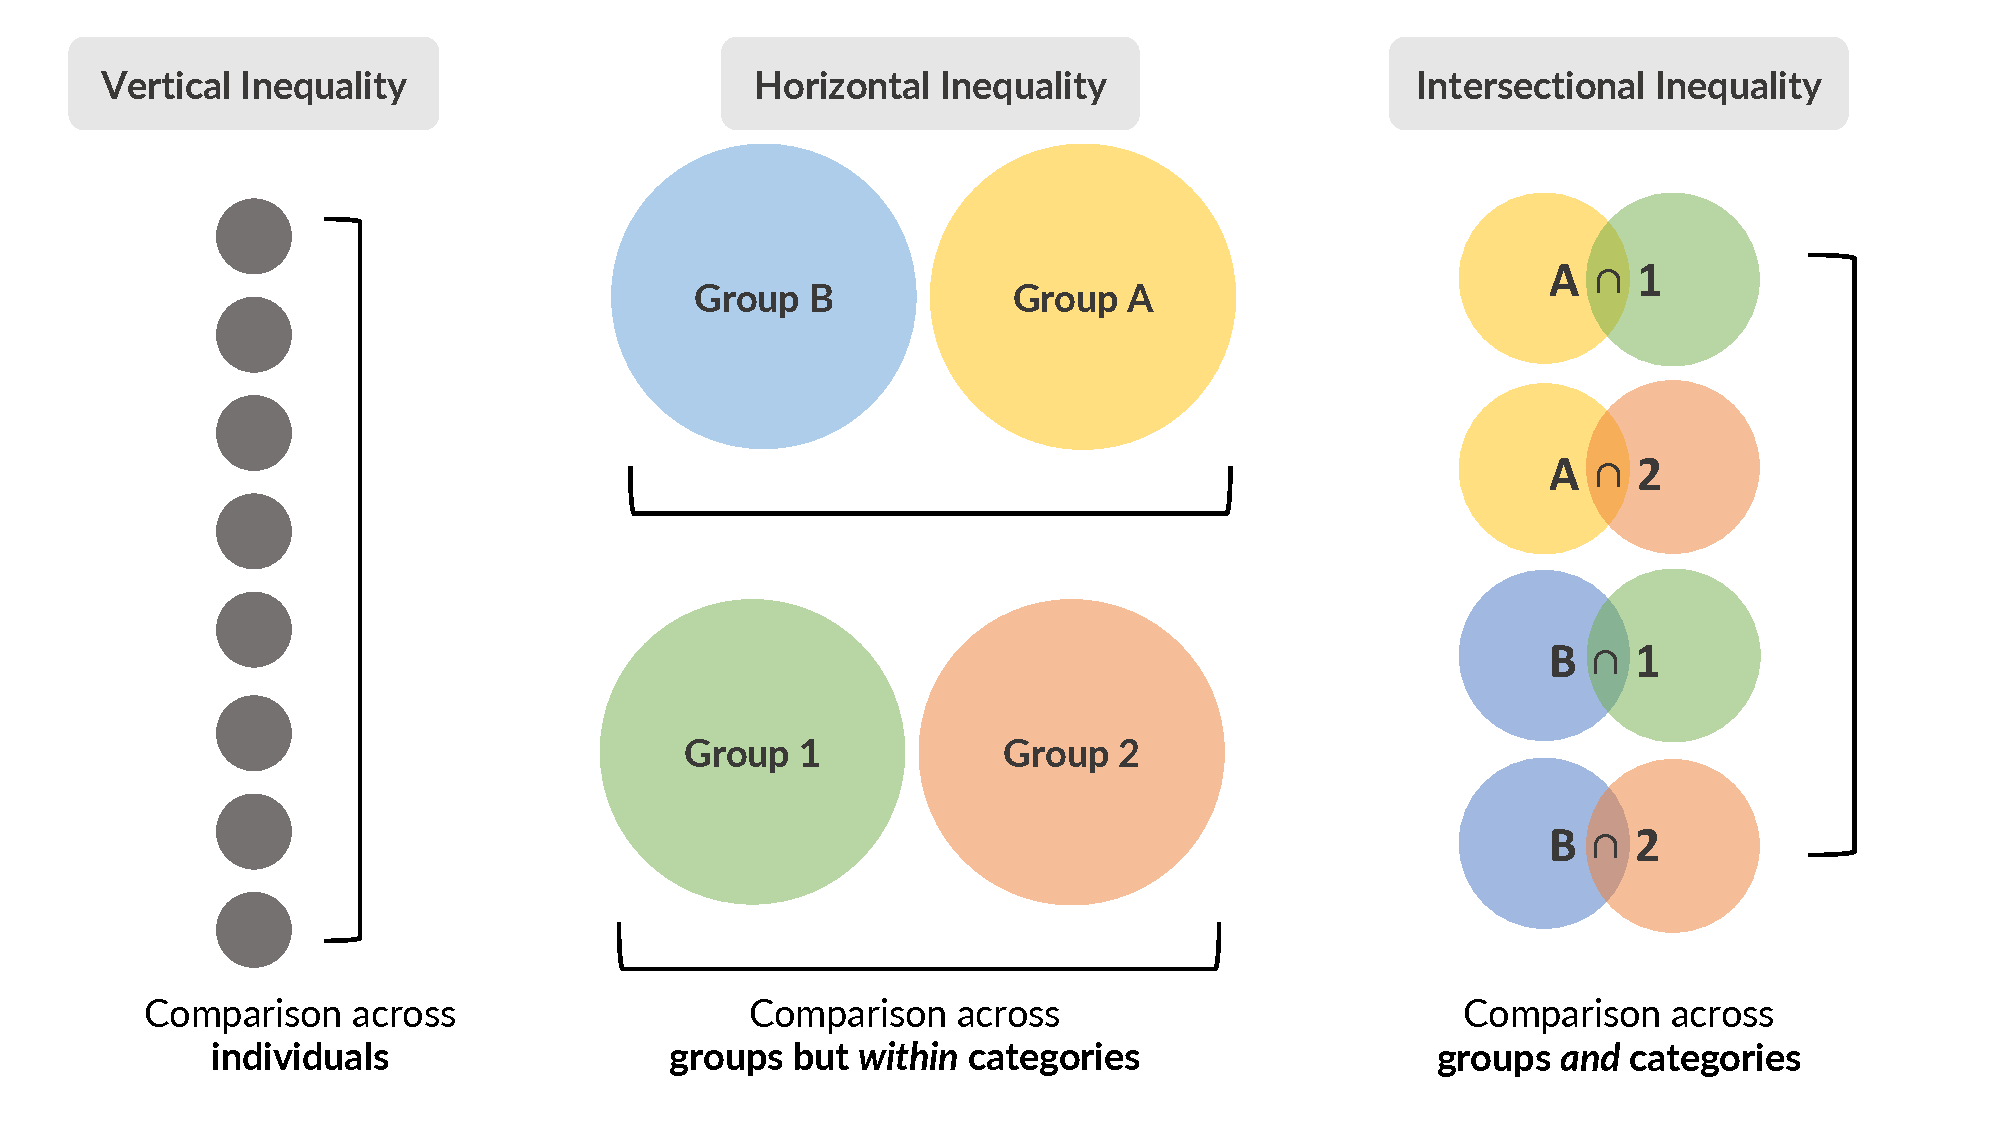
\includegraphics{latex/figures/intersectionality_framework.pdf} \caption[Concepts of inequality measurement]{Concepts of inequality measurements}\label{fig:intersectionality-framework}
\floatfoot{\textit{Notes:} Authors' own representation adopted from \cite{Lenhardt2015}}
\end{figure}

\begin{comment}
    % Figure 2 %%%%%%%%%%%%%%%%%%%%%%%%%%%%%%
\begin{figure}[htb]
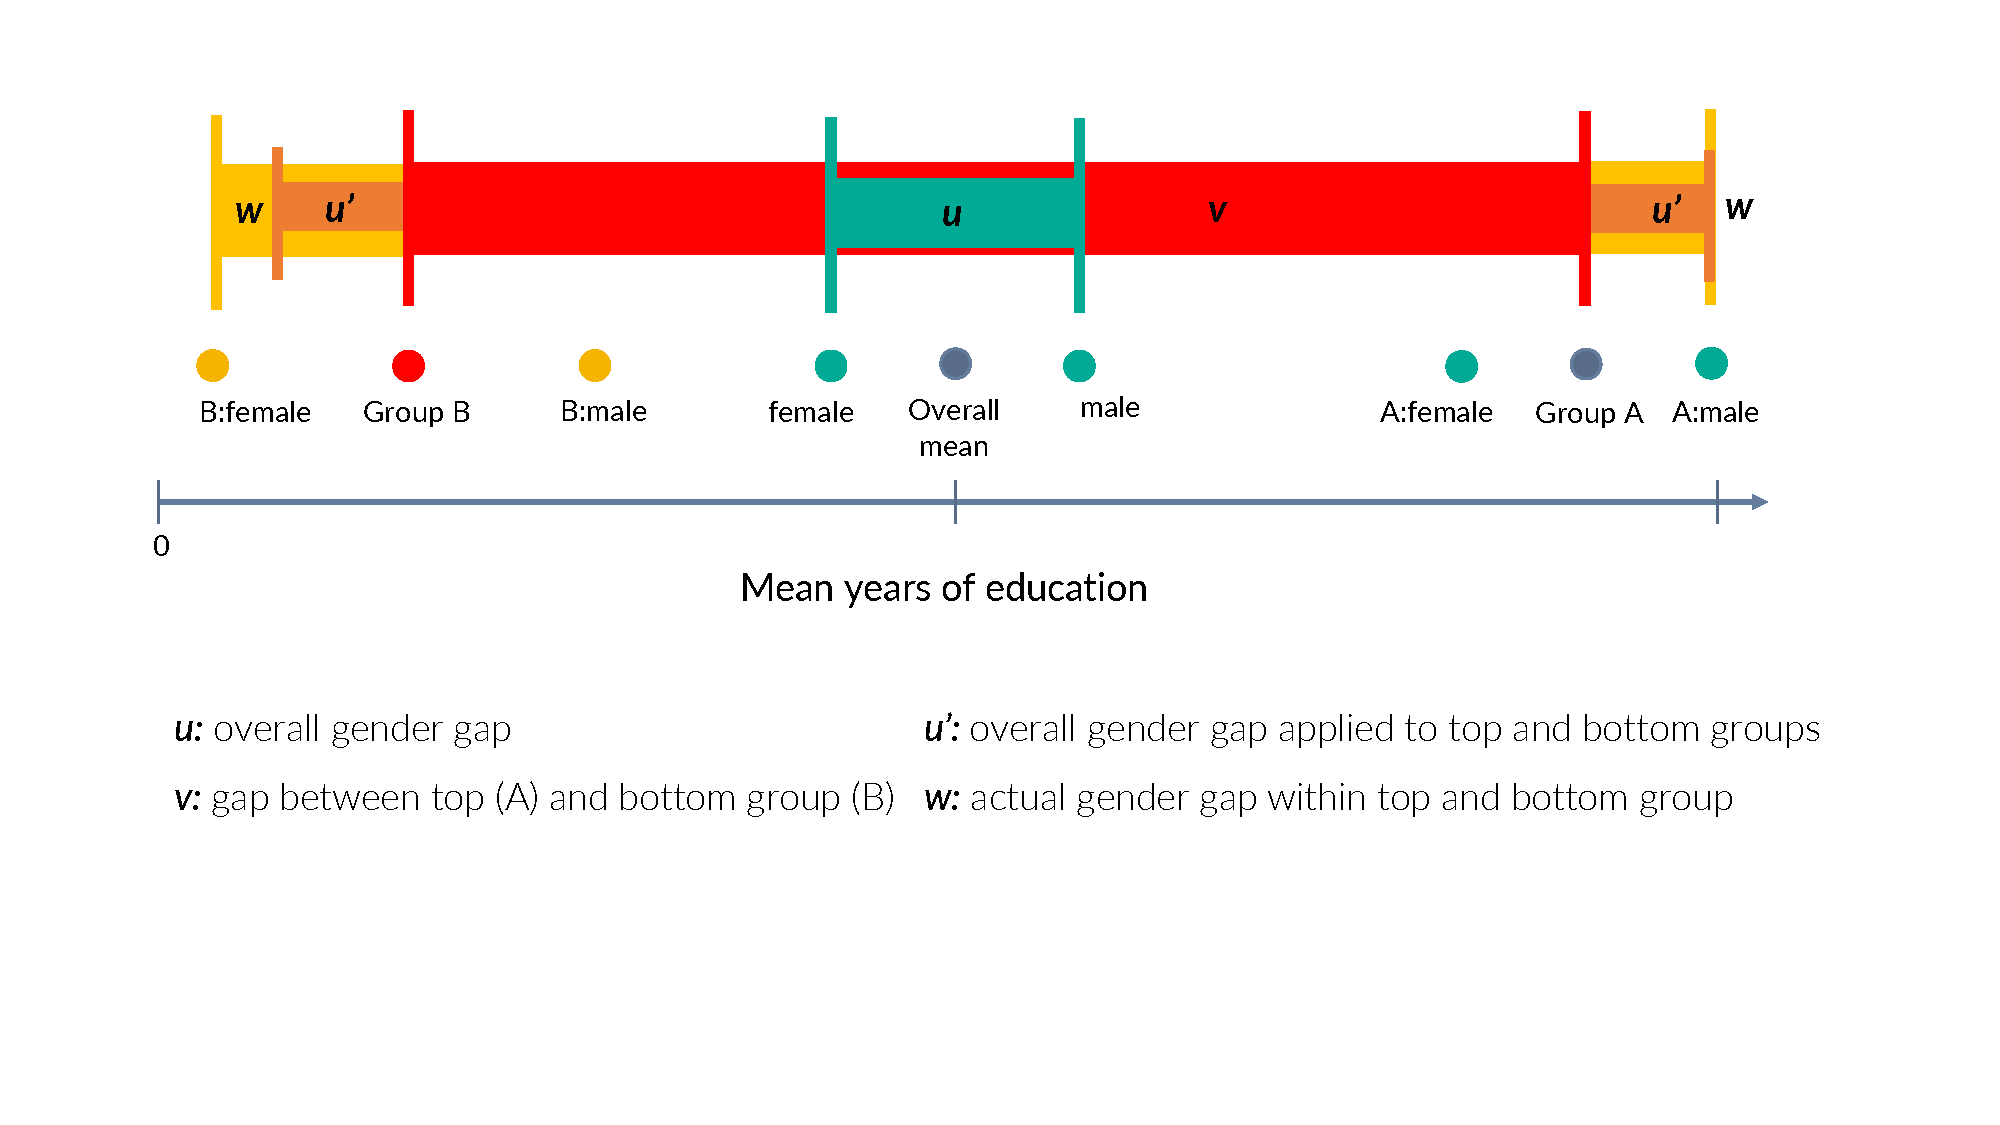
\includegraphics{latex/figures/surplus_schema.pdf} \caption[Schematic depiction of the total and counterfactual intersectional inequality]{Schematic depiction of the total and counterfactual intersectional inequality}\label{fig:surplus-schema}
\floatfoot{\textit{Notes:} Figure depicts a hypothetical scenario in which there are two categories with two groups each: female and male, group A and group B. In Group A, the observed gender gap equals the overall gender gap. In Group B, the observed gender gap is larger than the overall gender gap, resulting in differential intersectionality.} 
\end{figure}
\end{comment}


% Figure 3 %%%%%%%%%%%%%%%%%%%%%%%%%%%%%%

\begin{figure}[htb]
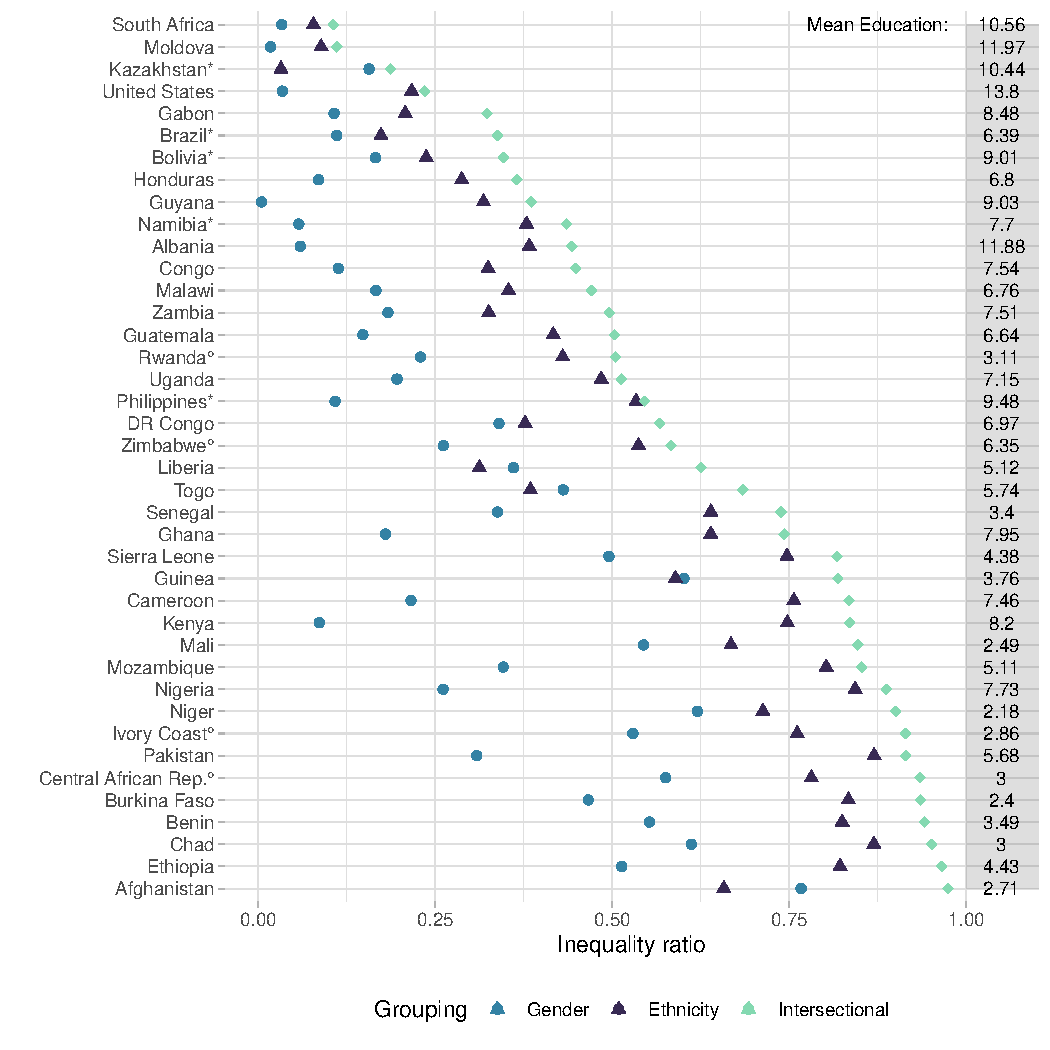
\includegraphics{latex/figures/world} 
\caption[Inequality in education (years of schooling) by gender, ethnicity and intersecting groups]{Inequality in education (years of schooling) by gender, ethnicity and intersecting groups}
\label{fig:world}
\floatfoot{\textit{Notes:} 
Aggregated data by country of $n=$2,689,279 individuals of the last available cohort; no mark means 1980 and younger cohort; countries marked with $*$ means 1970-1979 cohort; countries marked with \degree, the cohort born in 1969 and earlier was used. Using DHS sample weights, estimates show inequality ratios between groups with the lowest and highest average years of education. A value of 1 implies parity and a value of zero implies total inequality between the two most extreme groups. Sources: DHS 1992-2019 and US CPS 2019.} 
\end{figure}

% Figure 4 %%%%%%%%%%%%%%%%%%%%%%%%%%%%%%
\begin{figure}[htb]
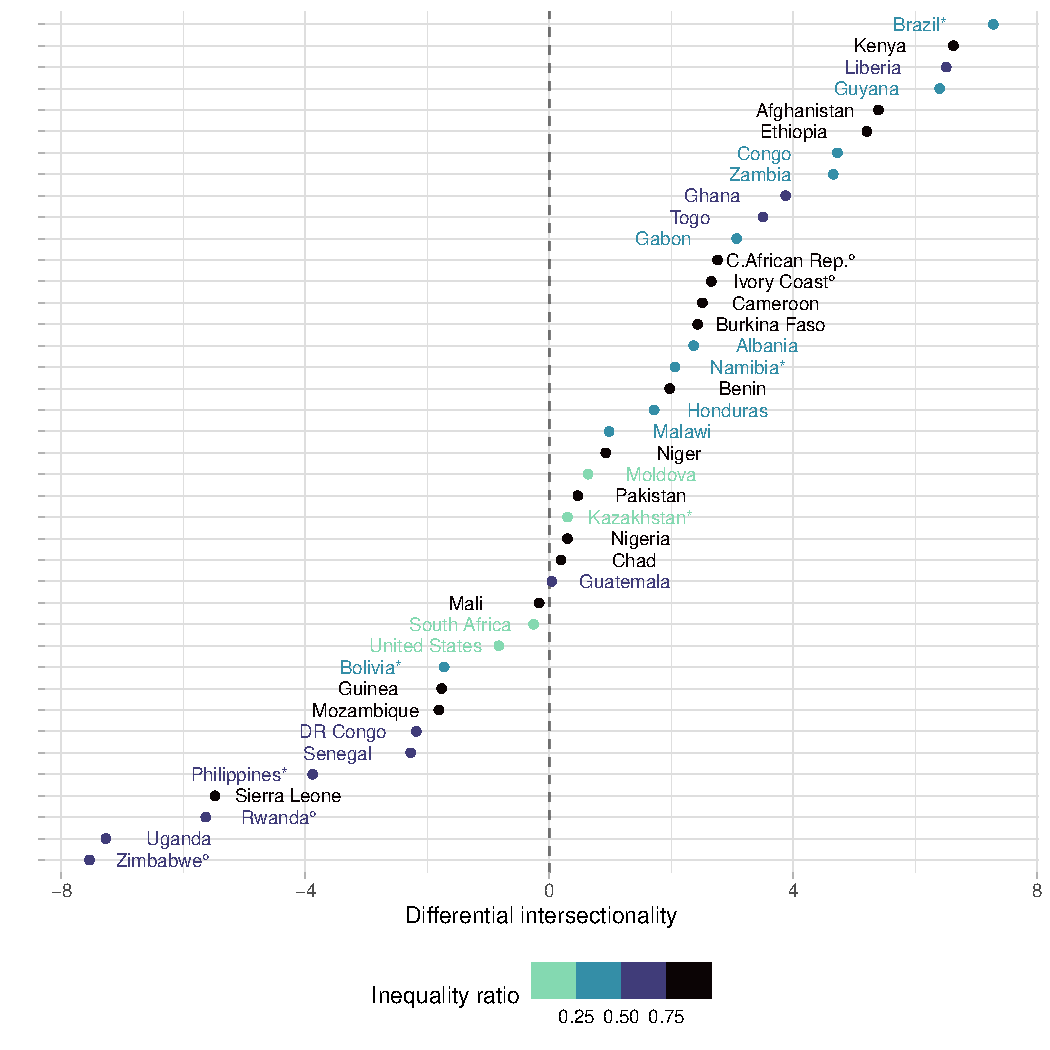
\includegraphics{latex/figures/diff-mech.pdf} 
\caption[Differential intersectionality (difference between counterfactual and total intersectional inequality]{Differential intersectionality (difference between counterfactual and total intersectional inequality}
\label{fig:diff-mech}
\floatfoot{\textit{Notes:} 
Aggregated data by country of $n=$2'689'279 individuals of the last available cohort; no mark means 1980 and younger cohort; countries marked with $*$ means 1970-1979 cohort; countries marked with \degree, the cohort born in 1969 and earlier was used. Estimates show the relative difference (in percent) between counterfactual and total intersectional inequality ratios. Values above zero indicate higher total intersectional inequality (lower IR) than would be the case with constant relative gender gaps across ethnic groups. Sources: DHS 1992-2019 and US CPS 2019.} \end{figure}

% Figure 5  %%%%%%%%%%%%%%%%%%%%%%%%%%%%%%
\begin{figure}[htb]
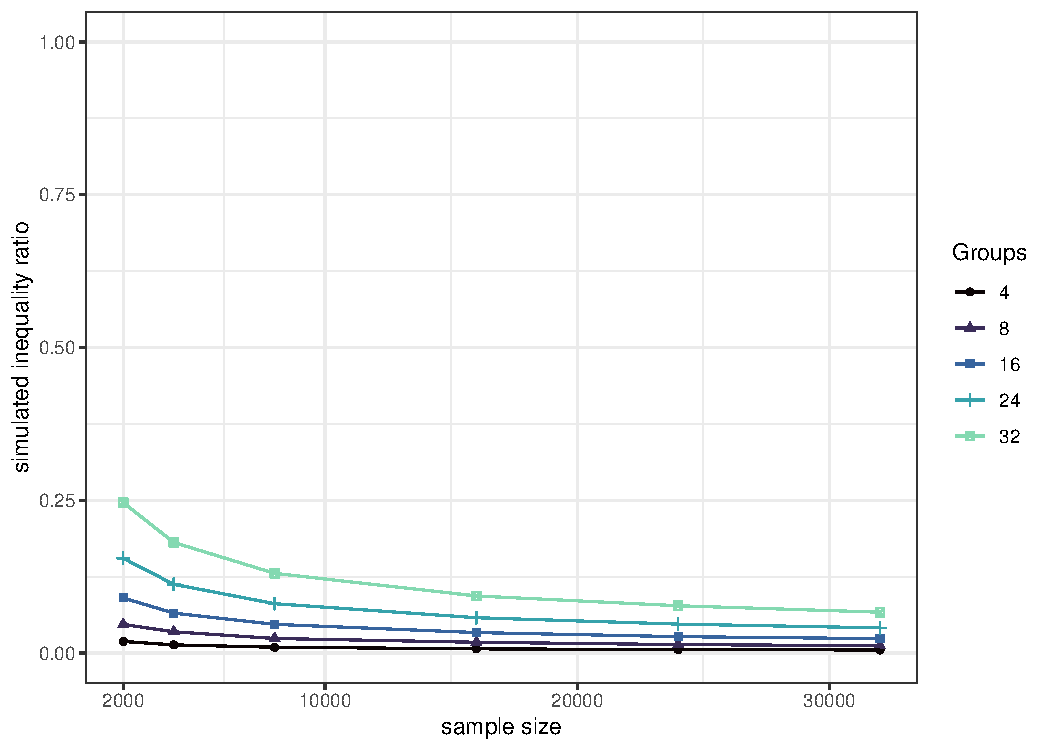
\includegraphics[width=0.9\linewidth,]{latex/figures/sensitivity-groups.pdf} \caption[Simulation with varying group size and sample size]{Simulation with varying group size and sample size}\label{fig:sensitivity}
\floatfoot{\textit{Notes:} Based on averages across 1000 iterations. Education data is drawn randomly from a truncated normal distribution bounded between 0 and 17 years with \(\mu=5.5\) and \(\sigma=3\), corresponding to the average education and standard deviation across all countries.} \end{figure}

\FloatBarrier
%%%%%%%%%%%%%%%%%%%%%%%%%%%%%%%%
% TABLES 
%%%%%%%%%%%%%%%%%%%%%%%%%%%%%%%%

% Table 1 %%%%%%%%%%%%%%%%%%%%%%%%%%%%%%
\begin{table}[htb]
\caption{\label{tab:tableone}Descriptive statistics by birth cohort brackets}
\centering

\begin{tabular}{lccc}
\toprule
\textbf{Characteristic} & \makecell[c]{\textbf{-1969}\ \ \\N = 30} & \makecell[c]{\textbf{1970-1979}\ \ \\N = 30} & \makecell[c]{\textbf{1980-}\ \ \\N = 30}\\
\midrule
Education (yrs) & 5.0 (3.4) & 5.6 (3.4) & 6.4 (3.3)\\
IR(gender) & 0.37 (0.21) & 0.33 (0.21) & 0.28 (0.20)\\
IR(ethnicity) & 0.60 (0.25) & 0.56 (0.25) & 0.53 (0.25)\\
IR(gender*ethnicity) & 0.73 (0.25) & 0.68 (0.27) & 0.64 (0.26)\\
Female (\%) & 0.62 (0.08) & 0.72 (0.07) & 0.73 (0.08)\\
No. of ethnic groups & 8 (4) & 8 (4) & 8 (4)\\
Sample size & 34,320 (133,352) & 22,700 (67,330) & 29,491 (104,609)\\
Group size low & 940 (1,766) & 1,019 (1,717) & 1,468 (2,952)\\
Group size high & 501 (579) & 411 (472) & 536 (1,037)\\
\bottomrule
\end{tabular}

\floatfoot{\textit{Notes:} Statistics report the Mean (SD); Median (IQR) for no. of ethnic groups, aggregated by birth cohort brackets; $n=$2,689,279 individuals older than 25 years and younger than the birth cohort of 1920. For comparability, only countries with observations in all three cohort brackets are included. Sources: DHS 1992-2019 and US CPS 2019.} 
\end{table}

% Table 2 %%%%%%%%%%%%%%%%%%%%%%%%%%%%%%
\begin{table}
\caption{Correlates of group inequality in education (OLS)\label{tab:ratios}}
\centering

\resizebox{\linewidth}{!}{
\tiny
\begin{tblr}[         %% tabularray outer open
]                     %% tabularray outer close
{                     %% tabularray inner open
colspec={Q[]Q[]Q[]Q[]Q[]Q[]Q[]},
cell{3}{1}={c=7}{},cell{15}{1}={c=7}{},cell{29}{1}={c=7}{},
cell{4}{1}={preto={\hspace{1em}}},
cell{5}{1}={preto={\hspace{1em}}},
cell{6}{1}={preto={\hspace{1em}}},
cell{7}{1}={preto={\hspace{1em}}},
cell{8}{1}={preto={\hspace{1em}}},
cell{9}{1}={preto={\hspace{1em}}},
cell{10}{1}={preto={\hspace{1em}}},
cell{11}{1}={preto={\hspace{1em}}},
cell{12}{1}={preto={\hspace{1em}}},
cell{13}{1}={preto={\hspace{1em}}},
cell{14}{1}={preto={\hspace{1em}}},
cell{16}{1}={preto={\hspace{1em}}},
cell{17}{1}={preto={\hspace{1em}}},
cell{18}{1}={preto={\hspace{1em}}},
cell{19}{1}={preto={\hspace{1em}}},
cell{20}{1}={preto={\hspace{1em}}},
cell{21}{1}={preto={\hspace{1em}}},
cell{22}{1}={preto={\hspace{1em}}},
cell{23}{1}={preto={\hspace{1em}}},
cell{24}{1}={preto={\hspace{1em}}},
cell{25}{1}={preto={\hspace{1em}}},
cell{26}{1}={preto={\hspace{1em}}},
cell{27}{1}={preto={\hspace{1em}}},
cell{28}{1}={preto={\hspace{1em}}},
cell{30}{1}={preto={\hspace{1em}}},
cell{31}{1}={preto={\hspace{1em}}},
cell{32}{1}={preto={\hspace{1em}}},
cell{33}{1}={preto={\hspace{1em}}},
cell{34}{1}={preto={\hspace{1em}}},
cell{35}{1}={preto={\hspace{1em}}},
cell{36}{1}={preto={\hspace{1em}}},
cell{37}{1}={preto={\hspace{1em}}},
cell{38}{1}={preto={\hspace{1em}}},
cell{39}{1}={preto={\hspace{1em}}},
cell{40}{1}={preto={\hspace{1em}}},
cell{41}{1}={preto={\hspace{1em}}},
cell{42}{1}={preto={\hspace{1em}}},
cell{43}{1}={preto={\hspace{1em}}},
cell{44}{1}={preto={\hspace{1em}}},
cell{45}{1}={preto={\hspace{1em}}},
cell{1}{1}={c=1,}{halign=c,},
cell{1}{2}={c=2,}{halign=c,},
cell{1}{4}={c=2,}{halign=c,},
cell{1}{6}={c=2,}{halign=c,},
column{1}={halign=l,},
column{2}={halign=c,},
column{3}={halign=c,},
column{4}={halign=c,},
column{5}={halign=c,},
column{6}={halign=c,},
column{7}={halign=c,},
hline{40}={1,2,3,4,5,6,7}{solid, 0.05em, black},
}                     %% tabularray inner close
\toprule
Outcome: & IR(gen:eth) &  & Counterfactual &  & Differential &  \\ \cmidrule[lr]{1-1}\cmidrule[lr]{2-3}\cmidrule[lr]{4-5}\cmidrule[lr]{6-7}
& (A) & (B) & (C) & (D) & (E) & (F) \\ \midrule %% TinyTableHeader
Panel A: Education Variables &&&&&& \\
Mean education (yrs)$^a$ & -0.06586*** & -0.06057*** & -0.06637*** & -0.06071*** & 0.00051     & 0.00014    \\
& (0.00609)   & (0.00898)   & (0.00595)   & (0.00857)   & (0.00107)   & (0.00149)  \\
Africa                   &             & 0.08308     &             & 0.08917     &             & -0.00609   \\
&             & (0.06875)   &             & (0.06591)   &             & (0.01078)  \\
Cohort 1970-1979$^c$     &             & -0.00590    &             & -0.00230    &             & -0.00360   \\
&             & (0.01515)   &             & (0.01227)   &             & (0.00692)  \\
Cohort 1980-$^c$         &             & 0.01667     &             & 0.01850     &             & -0.00183   \\
&             & (0.02341)   &             & (0.02147)   &             & (0.00785)  \\
(Intercept)              & 1.04552***  & 0.95336***  & 1.03457***  & 0.93423***  & 0.01094     & 0.01914    \\
& (0.03217)   & (0.08883)   & (0.03067)   & (0.08394)   & (0.00712)   & (0.01364)  \\
Adj. R2                  & 0.671       & 0.680       & 0.693       & 0.705       & -0.007      & -0.029     \\
Panel B: Sample Size &&&&&& \\
No. of ethnic groups     & 0.03251**   & 0.02387+    & 0.03242**   & 0.02303+    & 0.00008     & 0.00084    \\
& (0.01155)   & (0.01380)   & (0.01132)   & (0.01345)   & (0.00112)   & (0.00140)  \\
Sample size$^b$          & -0.00066*** & -0.00046**  & -0.00062*** & -0.00041*   & -0.00004*** & -0.00005** \\
& (0.00008)   & (0.00017)   & (0.00008)   & (0.00016)   & (0.00001)   & (0.00002)  \\
Africa                   &             & 0.16692     &             & 0.17974     &             & -0.01282   \\
&             & (0.10911)   &             & (0.10737)   &             & (0.01074)  \\
Cohort 1970-1979$^c$     &             & -0.05618*   &             & -0.05140*   &             & -0.00478   \\
&             & (0.02196)   &             & (0.02077)   &             & (0.00632)  \\
Cohort 1980-$^c$         &             & -0.06737*   &             & -0.06504*   &             & -0.00233   \\
&             & (0.03027)   &             & (0.02863)   &             & (0.00701)  \\
(Intercept)              & 0.42949***  & 0.41264***  & 0.41530***  & 0.39251***  & 0.01419     & 0.02013*   \\
& (0.09333)   & (0.08708)   & (0.09256)   & (0.08397)   & (0.00855)   & (0.00940)  \\
Adj. R2                  & 0.279       & 0.335       & 0.277       & 0.343       & -0.008      & -0.014     \\
Panel C: Group Size &&&&&& \\
Group size lowest        & -0.00001    & -0.00001    & -0.00001    & -0.00001    & -0.00001**  & -0.00001** \\
& (0.00002)   & (0.00001)   & (0.00002)   & (0.00001)   & (0.00000)   & (0.00000)  \\
Group size highest       & -0.00006    & 0.00001     & -0.00007    & 0.00001     & 0.00001+    & 0.00001    \\
& (0.00004)   & (0.00004)   & (0.00004)   & (0.00004)   & (0.00000)   & (0.00000)  \\
Africa                   &             & 0.28996**   &             & 0.29703**   &             & -0.00706   \\
&             & (0.10315)   &             & (0.10047)   &             & (0.00830)  \\
Cohort 1970-1979$^c$     &             & -0.03158    &             & -0.02834    &             & -0.00323   \\
&             & (0.02284)   &             & (0.02041)   &             & (0.00674)  \\
Cohort 1980-$^c$         &             & -0.03945    &             & -0.04024    &             & 0.00079    \\
&             & (0.03413)   &             & (0.03198)   &             & (0.00729)  \\
(Intercept)              & 0.70760***  & 0.49110***  & 0.69168***  & 0.46834***  & 0.01592**   & 0.02276*   \\
& (0.04686)   & (0.10587)   & (0.04736)   & (0.10255)   & (0.00491)   & (0.00891)  \\
Adj. R2                  & 0.034       & 0.234       & 0.029       & 0.243       & 0.065       & 0.047      \\
Num.Obs                  & 105         & 105         & 105         & 105         & 105         & 105        \\
Mean of DV               & 0.6635      & 0.6635      & 0.6495      & 0.6495      & 0.0139      & 0.0139     \\
\bottomrule
\end{tblr}
}
\floatfoot{\textit{Notes:} Aggregated country-cohort bracket level data of 40 countries; n=2'689'279 individuals 25 years and older born after 1920; cluster-robust standard errors on the country-level in parentheses. Sign. codes: $^*p<10\%$, $^{**}p<5\%$, $^{***}p<1\%$. \\
$^a$~Within-country-cohort weighted mean years of education with DHS sampling weights;\\
$^b$~Within-country-cohort (individual) Gini index takes on a value between 0 and 1;
$^c$~Corresponds to country-cohort sample size in units of 1000;\\
$^d$~Ref: Cohort -1969.}
\end{table}

\FloatBarrier
\clearpage


% Appendix %%%%%%%%%%%%%%%%%%%%%%%%%%%%%%
\begin{appendices}

% reset counter for figures and change labels
\setcounter{table}{0}
\renewcommand{\thetable}{\thesection\arabic{table}}
\setcounter{figure}{0}
\renewcommand\thefigure{\thesection\arabic{figure}} 
% Appendix  A %%%%%%%%%%%%%%%%%%%%%%%%%%%%%%
\begin{landscape}
\hypertarget{aggregated-data}{%
\section{Supplementary Tables}\label{aggregated-data}}
\renewcommand{\arraystretch}{0.8}% Tighter

\begingroup\fontsize{7}{9}\selectfont

\begin{ThreePartTable}
\begin{TableNotes}
\item \textit{Notes: } 
\item Education reports mean (sd); IR(G) reports inequality ratios between the group with the highest and lowest average education.
\end{TableNotes}
\begin{longtable}[t]{lccccccc}
\caption{\label{tab:aggregated}Education Inequality Ratios by Birth Cohort and Country for Gender and Ethnicity}\\
\toprule
Cohort & Education & IR(gender) & IR(eth) & IR(gen:eth) & IR(gen:eth)' & Differential & obs.\\
\midrule
\endfirsthead
\caption[]{Education Inequality Ratios by Birth Cohort and Country for Gender and Ethnicity \textit{(continued)}}\\
\toprule
Cohort & Education & IR(gender) & IR(eth) & IR(gen:eth) & IR(gen:eth)' & Differential & obs.\\
\midrule
\endhead

\endfoot
\bottomrule
\insertTableNotes
\endlastfoot
\addlinespace[0.3em]
\multicolumn{8}{l}{\textbf{Afghanistan}}\\
\hspace{1em}1970-1979 & 1.6 (3.62) & 0.81 & 0.63 & 0.99 & 0.93 & 0.07 & 10207\\
\hspace{1em}1980- & 2 (3.94) & 0.77 & 0.66 & 0.97 & 0.92 & 0.05 & 17528\\
\addlinespace[0.3em]
\multicolumn{8}{l}{\textbf{Albania}}\\
\hspace{1em}-1969 & 11.37 (4.04) & 0.06 & 0.21 & 0.27 & 0.26 & 0.01 & 10061\\
\hspace{1em}1970-1979 & 11.35 (4) & 0.01 & 0.25 & 0.30 & 0.25 & 0.04 & 7103\\
\hspace{1em}1980- & 12.14 (4.64) & 0.06 & 0.38 & 0.44 & 0.42 & 0.02 & 6443\\
\addlinespace[0.3em]
\multicolumn{8}{l}{\textbf{Benin}}\\
\hspace{1em}-1969 & 2.33 (4.06) & 0.54 & 0.93 & 0.97 & 0.97 & 0.01 & 17112\\
\hspace{1em}1970-1979 & 2.19 (3.7) & 0.56 & 0.85 & 0.94 & 0.94 & 0.01 & 19084\\
\hspace{1em}1980- & 2.86 (4.51) & 0.55 & 0.82 & 0.94 & 0.92 & 0.02 & 17737\\
\addlinespace[0.3em]
\multicolumn{8}{l}{\textbf{Bolivia}}\\
\hspace{1em}-1969 & 6.78 (5.1) & 0.17 & 0.33 & 0.43 & 0.45 & -0.02 & 8613\\
\hspace{1em}1970-1979 & 8.57 (4.92) & 0.17 & 0.24 & 0.35 & 0.36 & -0.02 & 6097\\
\addlinespace[0.3em]
\multicolumn{8}{l}{\textbf{Brazil}}\\
\hspace{1em}-1969 & 6.13 (4.23) & 0.08 & 0.25 & 0.32 & 0.31 & 0.01 & 9031\\
\hspace{1em}1970-1979 & 6.94 (3.88) & 0.11 & 0.17 & 0.34 & 0.27 & 0.07 & 894\\
\addlinespace[0.3em]
\multicolumn{8}{l}{\textbf{Burkina Faso}}\\
\hspace{1em}-1969 & 0.92 (2.8) & 0.50 & 0.76 & 0.90 & 0.88 & 0.02 & 18787\\
\hspace{1em}1970-1979 & 1.54 (3.52) & 0.56 & 0.76 & 0.89 & 0.90 & -0.01 & 11479\\
\hspace{1em}1980- & 1.96 (3.78) & 0.47 & 0.83 & 0.94 & 0.91 & 0.02 & 4883\\
\addlinespace[0.3em]
\multicolumn{8}{l}{\textbf{Cameroon}}\\
\hspace{1em}-1969 & 5.24 (4.54) & 0.31 & 0.89 & 0.95 & 0.93 & 0.03 & 13493\\
\hspace{1em}1970-1979 & 6.27 (4.58) & 0.25 & 0.79 & 0.91 & 0.84 & 0.06 & 13365\\
\hspace{1em}1980- & 7 (4.99) & 0.22 & 0.76 & 0.83 & 0.81 & 0.03 & 12775\\
\addlinespace[0.3em]
\multicolumn{8}{l}{\textbf{Central African Republic}}\\
\hspace{1em}-1969 & 2.45 (3.64) & 0.58 & 0.78 & 0.93 & 0.91 & 0.03 & 4616\\
\addlinespace[0.3em]
\multicolumn{8}{l}{\textbf{Chad}}\\
\hspace{1em}-1969 & 1.19 (2.84) & 0.72 & 0.87 & 0.98 & 0.96 & 0.02 & 9039\\
\hspace{1em}1970-1979 & 1.61 (3.3) & 0.70 & 0.83 & 0.96 & 0.95 & 0.01 & 7536\\
\hspace{1em}1980- & 2.44 (3.97) & 0.61 & 0.87 & 0.95 & 0.95 & 0.00 & 7733\\
\addlinespace[0.3em]
\multicolumn{8}{l}{\textbf{Congo}}\\
\hspace{1em}-1969 & 8.13 (4.38) & 0.28 & 0.34 & 0.52 & 0.53 & 0.00 & 5256\\
\hspace{1em}1970-1979 & 8.2 (3.75) & 0.19 & 0.19 & 0.38 & 0.35 & 0.03 & 7173\\
\hspace{1em}1980- & 8.32 (3.85) & 0.11 & 0.32 & 0.45 & 0.40 & 0.05 & 3930\\
\addlinespace[0.3em]
\multicolumn{8}{l}{\textbf{DR Congo}}\\
\hspace{1em}-1969 & 6.28 (4.59) & 0.46 & 0.43 & 0.70 & 0.69 & 0.01 & 6636\\
\hspace{1em}1970-1979 & 6.55 (4.45) & 0.35 & 0.39 & 0.56 & 0.61 & -0.05 & 9335\\
\hspace{1em}1980- & 6.59 (4.58) & 0.34 & 0.38 & 0.57 & 0.59 & -0.02 & 9355\\
\addlinespace[0.3em]
\multicolumn{8}{l}{\textbf{Ethiopia}}\\
\hspace{1em}-1969 & 1.48 (3.35) & 0.68 & 0.90 & NaN & 0.97 & NaN & 17072\\
\hspace{1em}1970-1979 & 2.34 (3.92) & 0.49 & 0.88 & 0.99 & 0.94 & 0.05 & 20654\\
\hspace{1em}1980- & 3.42 (4.69) & 0.51 & 0.82 & 0.97 & 0.91 & 0.05 & 18944\\
\addlinespace[0.3em]
\multicolumn{8}{l}{\textbf{Gabon}}\\
\hspace{1em}-1969 & 8.6 (3.8) & 0.24 & 0.29 & 0.58 & 0.46 & 0.13 & 2079\\
\hspace{1em}1970-1979 & 9.03 (3.87) & 0.20 & 0.33 & 0.49 & 0.46 & 0.03 & 2680\\
\hspace{1em}1980- & 9.81 (3.82) & 0.11 & 0.21 & 0.32 & 0.29 & 0.03 & 2506\\
\addlinespace[0.3em]
\multicolumn{8}{l}{\textbf{Ghana}}\\
\hspace{1em}-1969 & 6.14 (5.18) & 0.34 & 0.84 & 0.89 & 0.90 & 0.00 & 11024\\
\hspace{1em}1970-1979 & 6.88 (5.03) & 0.28 & 0.68 & 0.85 & 0.77 & 0.08 & 6505\\
\hspace{1em}1980- & 8.27 (5.17) & 0.18 & 0.64 & 0.74 & 0.70 & 0.04 & 5177\\
\addlinespace[0.3em]
\multicolumn{8}{l}{\textbf{Guatemala}}\\
\hspace{1em}-1969 & 4.26 (4.7) & 0.24 & 0.58 & 0.73 & 0.68 & 0.06 & 3783\\
\hspace{1em}1970-1979 & 4.92 (4.74) & 0.20 & 0.51 & 0.63 & 0.61 & 0.02 & 7471\\
\hspace{1em}1980- & 6.38 (4.9) & 0.15 & 0.42 & 0.50 & 0.50 & 0.00 & 10798\\
\addlinespace[0.3em]
\multicolumn{8}{l}{\textbf{Guinea}}\\
\hspace{1em}-1969 & 1.77 (4.24) & 0.62 & 0.62 & 0.84 & 0.86 & -0.01 & 4734\\
\hspace{1em}1970-1979 & 1.64 (3.95) & 0.72 & 0.58 & 0.88 & 0.88 & 0.00 & 4253\\
\hspace{1em}1980- & 3.03 (5.29) & 0.60 & 0.59 & 0.82 & 0.84 & -0.02 & 5811\\
\addlinespace[0.3em]
\multicolumn{8}{l}{\textbf{Guyana}}\\
\hspace{1em}-1969 & 7.92 (3.39) & 0.03 & 0.34 & 0.39 & 0.36 & 0.02 & 2065\\
\hspace{1em}1970-1979 & 8.64 (3.28) & 0.05 & 0.35 & 0.38 & 0.38 & 0.00 & 2327\\
\hspace{1em}1980- & 9.26 (3.09) & 0.00 & 0.32 & 0.39 & 0.32 & 0.06 & 1118\\
\addlinespace[0.3em]
\multicolumn{8}{l}{\textbf{Honduras}}\\
\hspace{1em}-1969 & 5.66 (4.57) & 0.11 & 0.39 & 0.54 & 0.46 & 0.08 & 4657\\
\hspace{1em}1970-1979 & 6.44 (4.3) & 0.06 & 0.32 & 0.38 & 0.37 & 0.01 & 7036\\
\hspace{1em}1980- & 7.51 (4.34) & 0.09 & 0.29 & 0.37 & 0.35 & 0.02 & 6768\\
\addlinespace[0.3em]
\multicolumn{8}{l}{\textbf{Ivory Coast}}\\
\hspace{1em}-1969 & 2.4 (3.91) & 0.53 & 0.76 & 0.91 & 0.89 & 0.03 & 6088\\
\addlinespace[0.3em]
\multicolumn{8}{l}{\textbf{Kazakhstan}}\\
\hspace{1em}-1969 & 10.77 (2.51) & 0.15 & 0.04 & 0.20 & 0.18 & 0.02 & 3533\\
\hspace{1em}1970-1979 & 10.77 (2.24) & 0.16 & 0.03 & 0.19 & 0.18 & 0.00 & 875\\
\addlinespace[0.3em]
\multicolumn{8}{l}{\textbf{Kenya}}\\
\hspace{1em}-1969 & 6.55 (4.3) & 0.25 & 0.84 & 0.93 & 0.88 & 0.05 & 19245\\
\hspace{1em}1970-1979 & 8.16 (3.94) & 0.13 & 0.80 & 0.88 & 0.83 & 0.05 & 18720\\
\hspace{1em}1980- & 8.84 (3.99) & 0.09 & 0.75 & 0.84 & 0.77 & 0.07 & 15797\\
\addlinespace[0.3em]
\multicolumn{8}{l}{\textbf{Liberia}}\\
\hspace{1em}-1969 & 4.39 (5.16) & 0.65 & 0.45 & 0.82 & 0.80 & 0.02 & 1402\\
\hspace{1em}1970-1979 & 4.55 (5.01) & 0.49 & 0.43 & 0.71 & 0.71 & 0.00 & 3187\\
\hspace{1em}1980- & 5.59 (5.12) & 0.36 & 0.31 & 0.63 & 0.56 & 0.07 & 3776\\
\addlinespace[0.3em]
\multicolumn{8}{l}{\textbf{Malawi}}\\
\hspace{1em}-1969 & 3.63 (3.65) & 0.40 & 0.66 & 0.84 & 0.80 & 0.04 & 15246\\
\hspace{1em}1970-1979 & 4.56 (3.96) & 0.34 & 0.56 & 0.72 & 0.71 & 0.02 & 21043\\
\hspace{1em}1980- & 6.32 (3.89) & 0.17 & 0.35 & 0.47 & 0.46 & 0.01 & 17567\\
\addlinespace[0.3em]
\multicolumn{8}{l}{\textbf{Mali}}\\
\hspace{1em}-1969 & 1.29 (3.11) & 0.53 & 0.66 & 0.88 & 0.84 & 0.03 & 21039\\
\hspace{1em}1970-1979 & 1.3 (3.2) & 0.54 & 0.62 & 0.84 & 0.83 & 0.01 & 15553\\
\hspace{1em}1980- & 2.01 (3.99) & 0.54 & 0.67 & 0.85 & 0.85 & 0.00 & 12203\\
\addlinespace[0.3em]
\multicolumn{8}{l}{\textbf{Moldova}}\\
\hspace{1em}-1969 & 11.5 (2.33) & 0.03 & 0.07 & 0.10 & 0.10 & 0.00 & 4121\\
\hspace{1em}1970-1979 & 11.54 (2.52) & 0.01 & 0.03 & 0.04 & 0.04 & 0.00 & 2320\\
\hspace{1em}1980- & 11.78 (2.74) & 0.02 & 0.09 & 0.11 & 0.10 & 0.01 & 258\\
\addlinespace[0.3em]
\multicolumn{8}{l}{\textbf{Mozambique}}\\
\hspace{1em}-1969 & 2.21 (2.94) & 0.53 & 0.83 & 0.89 & 0.92 & -0.03 & 8073\\
\hspace{1em}1970-1979 & 3.09 (3.49) & 0.38 & 0.82 & 0.87 & 0.89 & -0.02 & 5241\\
\hspace{1em}1980- & 3.96 (3.93) & 0.35 & 0.80 & 0.85 & 0.87 & -0.02 & 3993\\
\addlinespace[0.3em]
\multicolumn{8}{l}{\textbf{Namibia}}\\
\hspace{1em}-1969 & 6.57 (4.24) & 0.02 & 0.46 & 0.53 & 0.46 & 0.07 & 3882\\
\hspace{1em}1970-1979 & 8.11 (3.76) & 0.06 & 0.38 & 0.44 & 0.41 & 0.02 & 1868\\
\addlinespace[0.3em]
\multicolumn{8}{l}{\textbf{Niger}}\\
\hspace{1em}-1969 & 0.61 (2.15) & 0.40 & 0.82 & 0.88 & 0.90 & -0.01 & 13895\\
\hspace{1em}1970-1979 & 1.18 (2.83) & 0.54 & 0.73 & 0.85 & 0.88 & -0.03 & 4970\\
\hspace{1em}1980- & 1.17 (2.91) & 0.62 & 0.71 & 0.90 & 0.89 & 0.01 & 1142\\
\addlinespace[0.3em]
\multicolumn{8}{l}{\textbf{Nigeria}}\\
\hspace{1em}-1969 & 5.51 (5.68) & 0.37 & 0.90 & 0.95 & 0.94 & 0.02 & 18869\\
\hspace{1em}1970-1979 & 6.44 (5.69) & 0.30 & 0.89 & 0.94 & 0.92 & 0.02 & 35890\\
\hspace{1em}1980- & 7.16 (5.86) & 0.26 & 0.84 & 0.89 & 0.88 & 0.00 & 47233\\
\addlinespace[0.3em]
\multicolumn{8}{l}{\textbf{Pakistan}}\\
\hspace{1em}-1969 & 3.09 (4.61) & 0.56 & 0.87 & 0.99 & 0.94 & 0.05 & 2838\\
\hspace{1em}1970-1979 & 3.88 (4.95) & 0.51 & 0.80 & 0.94 & 0.90 & 0.04 & 5525\\
\hspace{1em}1980- & 4.49 (4.96) & 0.31 & 0.87 & 0.91 & 0.91 & 0.00 & 5456\\
\addlinespace[0.3em]
\multicolumn{8}{l}{\textbf{Philippines}}\\
\hspace{1em}-1969 & 8.92 (4.21) & 0.07 & 0.61 & 0.63 & 0.64 & -0.01 & 7089\\
\hspace{1em}1970-1979 & 9.9 (4) & 0.11 & 0.53 & 0.55 & 0.58 & -0.04 & 4765\\
\addlinespace[0.3em]
\multicolumn{8}{l}{\textbf{Rwanda}}\\
\hspace{1em}-1969 & 2.53 (3.28) & 0.23 & 0.43 & 0.50 & 0.56 & -0.06 & 4364\\
\addlinespace[0.3em]
\multicolumn{8}{l}{\textbf{Senegal}}\\
\hspace{1em}-1969 & 2.39 (4.23) & 0.41 & 0.56 & 0.77 & 0.74 & 0.02 & 23810\\
\hspace{1em}1970-1979 & 2.92 (4.35) & 0.40 & 0.60 & 0.75 & 0.76 & 0.00 & 25146\\
\hspace{1em}1980- & 3.59 (4.86) & 0.34 & 0.64 & 0.74 & 0.76 & -0.02 & 35847\\
\addlinespace[0.3em]
\multicolumn{8}{l}{\textbf{Sierra Leone}}\\
\hspace{1em}-1969 & 2.87 (4.88) & 0.53 & 0.82 & 0.93 & 0.91 & 0.02 & 6013\\
\hspace{1em}1970-1979 & 2.44 (4.37) & 0.51 & 0.86 & 0.91 & 0.93 & -0.02 & 12515\\
\hspace{1em}1980- & 3.87 (5.1) & 0.50 & 0.75 & 0.82 & 0.87 & -0.05 & 17503\\
\addlinespace[0.3em]
\multicolumn{8}{l}{\textbf{South Africa}}\\
\hspace{1em}-1969 & 8.78 (4.31) & 0.08 & 0.26 & 0.33 & 0.32 & 0.01 & 1154\\
\hspace{1em}1970-1979 & 10.02 (3.58) & 0.01 & 0.10 & 0.11 & 0.11 & 0.00 & 2537\\
\hspace{1em}1980- & 10.85 (2.69) & 0.03 & 0.08 & 0.11 & 0.11 & 0.00 & 4221\\
\addlinespace[0.3em]
\multicolumn{8}{l}{\textbf{Togo}}\\
\hspace{1em}-1969 & 3.34 (4.1) & 0.58 & 0.63 & 0.87 & 0.84 & 0.02 & 7482\\
\hspace{1em}1970-1979 & 3.8 (4.11) & 0.54 & 0.63 & 0.85 & 0.83 & 0.03 & 4954\\
\hspace{1em}1980- & 5.38 (4.7) & 0.43 & 0.38 & 0.68 & 0.65 & 0.04 & 4077\\
\addlinespace[0.3em]
\multicolumn{8}{l}{\textbf{Uganda}}\\
\hspace{1em}-1969 & 4.17 (3.92) & 0.42 & 0.63 & 0.77 & 0.79 & -0.01 & 7065\\
\hspace{1em}1970-1979 & 5.11 (4.29) & 0.31 & 0.53 & 0.65 & 0.68 & -0.03 & 7187\\
\hspace{1em}1980- & 6.91 (4.5) & 0.20 & 0.48 & 0.51 & 0.59 & -0.07 & 10809\\
\addlinespace[0.3em]
\multicolumn{8}{l}{\textbf{United States}}\\
\hspace{1em}-1969 & 13.23 (2.87) & 0.01 & 0.28 & 0.28 & 0.29 & 0.00 & 739514\\
\hspace{1em}1970-1979 & 13.5 (2.91) & 0.03 & 0.26 & 0.28 & 0.28 & -0.01 & 376732\\
\hspace{1em}1980- & 13.65 (2.64) & 0.03 & 0.22 & 0.24 & 0.24 & -0.01 & 580778\\
\addlinespace[0.3em]
\multicolumn{8}{l}{\textbf{Zambia}}\\
\hspace{1em}-1969 & 6.44 (4.05) & 0.30 & 0.47 & 0.64 & 0.62 & 0.02 & 14043\\
\hspace{1em}1970-1979 & 6.77 (3.87) & 0.22 & 0.38 & 0.48 & 0.52 & -0.03 & 13487\\
\hspace{1em}1980- & 7.4 (4.01) & 0.18 & 0.33 & 0.50 & 0.45 & 0.05 & 10080\\
\addlinespace[0.3em]
\multicolumn{8}{l}{\textbf{Zimbabwe}}\\
\hspace{1em}-1969 & 6.07 (4.02) & 0.26 & 0.54 & 0.58 & 0.66 & -0.08 & 4506\\*
\end{longtable}
\end{ThreePartTable}
\endgroup{}

\clearpage
\begingroup\fontsize{7}{9}\selectfont

\begin{ThreePartTable}
\begin{TableNotes}
\item \textit{Notes: } 
\item Table reports the names of the groups with the lowest and highest average education used for inequality ratios.
\end{TableNotes}
\begin{longtable}[t]{lllllll}
\caption{\label{tab:groupnames}Names of Groups with the Lowest and Highest Education by Birth Cohort}\\
\toprule
Cohort & Gender low & Gender high & Ethnicity low & Ethnicity high & Intersect. low & Intersect. high\\
\midrule
\endfirsthead
\caption[]{Names of Groups with the Lowest and Highest Education by Birth Cohort \textit{(continued)}}\\
\toprule
Cohort & Gender low & Gender high & Ethnicity low & Ethnicity high & Intersect. low & Intersect. high\\
\midrule
\endhead

\endfoot
\bottomrule
\insertTableNotes
\endlastfoot
\addlinespace[0.3em]
\multicolumn{7}{l}{\textbf{Afghanistan}}\\
\hspace{1em}1970-1979 & F & M & nuristani & tajik & F:nuristani & M:tajik\\
\hspace{1em}1980- & F & M & nuristani & uzbek & F:nuristani & M:uzbek\\
\addlinespace[0.3em]
\multicolumn{7}{l}{\textbf{Albania}}\\
\hspace{1em}-1969 & F & M & other & albanian & F:other & M:albanian\\
\hspace{1em}1970-1979 & F & M & other & albanian & M:other & M:albanian\\
\hspace{1em}1980- & F & M & other & albanian & M:other & M:albanian\\
\addlinespace[0.3em]
\multicolumn{7}{l}{\textbf{Benin}}\\
\hspace{1em}-1969 & F & M & Peulh & Yoruba & F:Peulh & M:Yoruba\\
\hspace{1em}1970-1979 & F & M & Peulh & Other & F:Peulh & M:Fon\\
\hspace{1em}1980- & F & M & Peulh & Fon & F:Peulh & M:Adja\\
\addlinespace[0.3em]
\multicolumn{7}{l}{\textbf{Bolivia}}\\
\hspace{1em}-1969 & F & M & quechua & none & F:quechua & M:none\\
\hspace{1em}1970-1979 & F & M & quechua & none & F:quechua & M:aymara\\
\addlinespace[0.3em]
\multicolumn{7}{l}{\textbf{Brazil}}\\
\hspace{1em}-1969 & M & F & black/mixed/o... & white & M:black/mixed... & F:white\\
\hspace{1em}1970-1979 & M & F & black/mixed/o... & white & M:black/mixed... & M:white\\
\addlinespace[0.3em]
\multicolumn{7}{l}{\textbf{Burkina Faso}}\\
\hspace{1em}-1969 & F & M & Gurma & Gurunsi & F:Gurma & M:Bobo\\
\hspace{1em}1970-1979 & F & M & Fulfuldé/Peul & Gurunsi & F:Fulfuldé/Peul & M:Bobo\\
\hspace{1em}1980- & F & M & Gurma & Bobo & F:Gurma & M:Lobi\\
\addlinespace[0.3em]
\multicolumn{7}{l}{\textbf{Cameroon}}\\
\hspace{1em}-1969 & F & M & Arab-choa/Peu... & Côtier/Ngoe/O... & F:Biu-Mandara & M:Côtier/Ngoe...\\
\hspace{1em}1970-1979 & F & M & Arab-choa/Peu... & Beti/Bassa/Mbam & F:Biu-Mandara & M:Beti/Bassa/...\\
\hspace{1em}1980- & F & M & Arab-choa/Peu... & Côtier/Ngoe/O... & F:Arab-choa/P... & M:Beti/Bassa/...\\
\addlinespace[0.3em]
\multicolumn{7}{l}{\textbf{Central African Republic}}\\
\hspace{1em}-1969 & F & M & haoussa & yakoma-sango & F:haoussa & M:yakoma-sango\\
\addlinespace[0.3em]
\multicolumn{7}{l}{\textbf{Chad}}\\
\hspace{1em}-1969 & F & M & gorane & sara (ngambay... & F:gorane & M:sara (ngamb...\\
\hspace{1em}1970-1979 & F & M & kanembou / bo... & sara (ngambay... & F:kanembou / ... & M:sara (ngamb...\\
\hspace{1em}1980- & F & M & kanembou / bo... & sara (ngambay... & F:kanembou / ... & M:sara (ngamb...\\
\addlinespace[0.3em]
\multicolumn{7}{l}{\textbf{Congo}}\\
\hspace{1em}-1969 & F & M & Other non-Con... & Mbohhi & F:Other non-C... & M:Mbohhi\\
\hspace{1em}1970-1979 & F & M & Other Congolese & Mbohhi & F:Other non-C... & M:Mbeti\\
\hspace{1em}1980- & F & M & Other non-Con... & Mbohhi & F:Other non-C... & M:Mbeti\\
\addlinespace[0.3em]
\multicolumn{7}{l}{\textbf{DR Congo}}\\
\hspace{1em}-1969 & F & M & uele lac albert & bakongo & F:ubangi and ... & M:bakongo\\
\hspace{1em}1970-1979 & F & M & uele lac albert & bakongo & F:uele lac al... & M:bas-kasai a...\\
\hspace{1em}1980- & F & M & uele lac albert & bakongo & F:ubangi and ... & M:cuvette cen...\\
\addlinespace[0.3em]
\multicolumn{7}{l}{\textbf{Ethiopia}}\\
\hspace{1em}-1969 & F & M & Affar & Welaita & F:Gumuz & M:Welaita\\
\hspace{1em}1970-1979 & F & M & Affar & Guragie & F:Berta & M:Nuer\\
\hspace{1em}1980- & F & M & Affar & Nuer & F:Affar & M:Nuer\\
\addlinespace[0.3em]
\multicolumn{7}{l}{\textbf{Gabon}}\\
\hspace{1em}-1969 & F & M & kota-kele & fang & F:kota-kele & M:fang\\
\hspace{1em}1970-1979 & F & M & kota-kele & fang & F:kota-kele & M:fang\\
\hspace{1em}1980- & F & M & kota-kele & fang & F:kota-kele & M:fang\\
\addlinespace[0.3em]
\multicolumn{7}{l}{\textbf{Ghana}}\\
\hspace{1em}-1969 & F & M & gruma & ga/dangme & F:gruma & M:ga/dangme\\
\hspace{1em}1970-1979 & F & M & gruma & akan & F:gruma & M:akan\\
\hspace{1em}1980- & F & M & gruma & akan & F:gruma & M:akan\\
\addlinespace[0.3em]
\multicolumn{7}{l}{\textbf{Guatemala}}\\
\hspace{1em}-1969 & F & M & maya/other & ladina/mestiza & F:maya/other & M:ladina/mestiza\\
\hspace{1em}1970-1979 & F & M & maya/other & ladina/mestiza & F:maya/other & M:ladina/mestiza\\
\hspace{1em}1980- & F & M & maya/other & ladina/mestiza & F:maya/other & M:ladina/mestiza\\
\addlinespace[0.3em]
\multicolumn{7}{l}{\textbf{Guinea}}\\
\hspace{1em}-1969 & F & M & peulh & soussou & F:peulh & M:other\\
\hspace{1em}1970-1979 & F & M & peulh & soussou & F:guerzé & M:soussou\\
\hspace{1em}1980- & F & M & peulh & other & F:peulh & M:other\\
\addlinespace[0.3em]
\multicolumn{7}{l}{\textbf{Guyana}}\\
\hspace{1em}-1969 & M & F & amerindian & african & F:amerindian & F:african\\
\hspace{1em}1970-1979 & M & F & amerindian & african & F:amerindian & F:african\\
\hspace{1em}1980- & M & F & amerindian & african & M:amerindian & F:african\\
\addlinespace[0.3em]
\multicolumn{7}{l}{\textbf{Honduras}}\\
\hspace{1em}-1969 & M & F & None & Other & M:None & F:Other\\
\hspace{1em}1970-1979 & M & F & None & Other & M:None & F:Other\\
\hspace{1em}1980- & M & F & None & Other & M:None & F:Other\\
\addlinespace[0.3em]
\multicolumn{7}{l}{\textbf{Ivory Coast}}\\
\hspace{1em}-1969 & F & M & Burkina-Faso & Ivorian & F:Burkina-Faso & M:Ivorian\\
\addlinespace[0.3em]
\multicolumn{7}{l}{\textbf{Kazakhstan}}\\
\hspace{1em}-1969 & M & F & Other & Russian & M:Other & F:Russian\\
\hspace{1em}1970-1979 & M & F & Other & Russian & M:Russian & F:Russian\\
\addlinespace[0.3em]
\multicolumn{7}{l}{\textbf{Kenya}}\\
\hspace{1em}-1969 & F & M & turkana & kikuyu & F:turkana & M:kikuyu\\
\hspace{1em}1970-1979 & F & M & somali & kikuyu & F:somali & M:kisii\\
\hspace{1em}1980- & F & M & somali & kisii & F:somali & M:kisii\\
\addlinespace[0.3em]
\multicolumn{7}{l}{\textbf{Liberia}}\\
\hspace{1em}-1969 & F & M & Kpelle & Grebo & F:Kpelle & M:Other Kru\\
\hspace{1em}1970-1979 & F & M & Kpelle & Other Kru & F:Kpelle & M:Other Kru\\
\hspace{1em}1980- & F & M & Kpelle & Other & F:Kpelle & M:Grebo\\
\addlinespace[0.3em]
\multicolumn{7}{l}{\textbf{Malawi}}\\
\hspace{1em}-1969 & F & M & sena & tumbuka & F:sena & M:tumbuka\\
\hspace{1em}1970-1979 & F & M & sena & tumbuka & F:sena & M:tumbuka\\
\hspace{1em}1980- & F & M & sena & tumbuka & F:sena & M:nkondhe\\
\addlinespace[0.3em]
\multicolumn{7}{l}{\textbf{Mali}}\\
\hspace{1em}-1969 & F & M & dogon & malinke & F:dogon & M:malinke\\
\hspace{1em}1970-1979 & F & M & tamacheck & malinke & F:dogon & M:malinke\\
\hspace{1em}1980- & F & M & tamacheck & bobo & F:tamacheck & M:bobo\\
\addlinespace[0.3em]
\multicolumn{7}{l}{\textbf{Moldova}}\\
\hspace{1em}-1969 & M & F & moldovan & other & M:moldovan & F:other\\
\hspace{1em}1970-1979 & M & F & moldovan & other & M:other & F:other\\
\hspace{1em}1980- & M & F & moldovan & other & F:moldovan & F:other\\
\addlinespace[0.3em]
\multicolumn{7}{l}{\textbf{Mozambique}}\\
\hspace{1em}-1969 & F & M & Chewa & Portuguese & F:Sena & F:Portuguese\\
\hspace{1em}1970-1979 & F & M & Chewa & Portuguese & F:Chewa & M:Portuguese\\
\hspace{1em}1980- & F & M & Chewa & Portuguese & F:Chewa & M:Portuguese\\
\addlinespace[0.3em]
\multicolumn{7}{l}{\textbf{Namibia}}\\
\hspace{1em}-1969 & M & F & kavango langu... & afrikaans & F:kavango lan... & M:afrikaans\\
\hspace{1em}1970-1979 & M & F & kavango langu... & afrikaans & F:kavango lan... & M:afrikaans\\
\addlinespace[0.3em]
\multicolumn{7}{l}{\textbf{Niger}}\\
\hspace{1em}-1969 & F & M & Touareg/Touar... & Other & F:Touareg/Tou... & M:Other\\
\hspace{1em}1970-1979 & F & M & Touareg/Touar... & Other & F:Touareg/Tou... & M:Djerma\\
\hspace{1em}1980- & F & M & Touareg/Touar... & Djerma & F:Kanouri & M:Djerma\\
\addlinespace[0.3em]
\multicolumn{7}{l}{\textbf{Nigeria}}\\
\hspace{1em}-1969 & F & M & Fulani & Yoruba & F:Fulani & M:Ijaw/Izon\\
\hspace{1em}1970-1979 & F & M & Fulani & Yoruba & F:Fulani & M:Ijaw/Izon\\
\hspace{1em}1980- & F & M & Fulani & Igbo & F:Fulani & M:Yoruba\\
\addlinespace[0.3em]
\multicolumn{7}{l}{\textbf{Pakistan}}\\
\hspace{1em}-1969 & F & M & Barauhi & Urdu & F:Balochi & M:Urdu\\
\hspace{1em}1970-1979 & F & M & Barauhi & Urdu & F:Barauhi & M:Urdu\\
\hspace{1em}1980- & F & M & Barauhi & Urdu & F:Barauhi & M:Urdu\\
\addlinespace[0.3em]
\multicolumn{7}{l}{\textbf{Philippines}}\\
\hspace{1em}-1969 & M & F & maguindanaon & tagalog & F:maguindanaon & F:tagalog\\
\hspace{1em}1970-1979 & M & F & maguindanaon & tagalog & F:maguindanaon & F:tagalog\\
\addlinespace[0.3em]
\multicolumn{7}{l}{\textbf{Rwanda}}\\
\hspace{1em}-1969 & F & M & hutu & tutsi/other & F:hutu & M:tutsi/other\\
\addlinespace[0.3em]
\multicolumn{7}{l}{\textbf{Senegal}}\\
\hspace{1em}-1969 & F & M & Poular & Other & F:Poular & M:Diola\\
\hspace{1em}1970-1979 & F & M & Poular & Diola & F:Poular & M:Diola\\
\hspace{1em}1980- & F & M & Poular & Diola & F:Poular & M:Diola\\
\addlinespace[0.3em]
\multicolumn{7}{l}{\textbf{Sierra Leone}}\\
\hspace{1em}-1969 & F & M & Fullah & Creole & F:Kono & M:Creole\\
\hspace{1em}1970-1979 & F & M & Other & Creole & F:Other & M:Creole\\
\hspace{1em}1980- & F & M & Other & Creole & F:Other & M:Creole\\
\addlinespace[0.3em]
\multicolumn{7}{l}{\textbf{South Africa}}\\
\hspace{1em}-1969 & M & F & black/african & white/coloure... & M:black/african & M:white/colou...\\
\hspace{1em}1970-1979 & M & F & black/african & white/coloure... & M:black/african & M:white/colou...\\
\hspace{1em}1980- & M & F & black/african & white/coloure... & M:black/african & F:white/colou...\\
\addlinespace[0.3em]
\multicolumn{7}{l}{\textbf{Togo}}\\
\hspace{1em}-1969 & F & M & para-gourma/akan & akposso/akebou & F:para-gourma... & M:adja-ewe/mina\\
\hspace{1em}1970-1979 & F & M & para-gourma/akan & akposso/akebou & F:para-gourma... & M:akposso/akebou\\
\hspace{1em}1980- & F & M & para-gourma/akan & kabye/tem & F:para-gourma... & M:ana-ife\\
\addlinespace[0.3em]
\multicolumn{7}{l}{\textbf{Uganda}}\\
\hspace{1em}-1969 & F & M & Ruanda-Rundi & baganda & F:moru-madi & M:baganda\\
\hspace{1em}1970-1979 & F & M & moru-madi & baganda & F:moru-madi & M:langi\\
\hspace{1em}1980- & F & M & Ruanda-Rundi & baganda & F:alur-acholi & M:alur-acholi\\
\addlinespace[0.3em]
\multicolumn{7}{l}{\textbf{United States}}\\
\hspace{1em}-1969 & M & F & Other race & Japanese & M:Other race & F:Japanese\\
\hspace{1em}1970-1979 & M & F & Other race & Japanese & M:Other race & M:Japanese\\
\hspace{1em}1980- & M & F & Other race & Chinese & M:Other race & F:Chinese\\
\addlinespace[0.3em]
\multicolumn{7}{l}{\textbf{Zambia}}\\
\hspace{1em}-1969 & F & M & mbunda & lozi & F:mbunda & M:namwanga\\
\hspace{1em}1970-1979 & F & M & mbunda & namwanga & F:mbunda & M:namwanga\\
\hspace{1em}1980- & F & M & mbunda & lozi & F:mbunda & M:other\\
\addlinespace[0.3em]
\multicolumn{7}{l}{\textbf{Zimbabwe}}\\
\hspace{1em}-1969 & F & M & black & white & F:black & F:white\\*
\end{longtable}
\end{ThreePartTable}
\endgroup{}

\end{landscape}
\begingroup\fontsize{7}{9}\selectfont

\begin{longtable}[t]{>{\raggedright\arraybackslash}p{7em}>{\raggedright\arraybackslash}p{6em}>{\raggedright\arraybackslash}p{18em}r}
\caption{\label{tab:years-ethnicity}Survey Years and Ethnic Groups}\\
\toprule
Country & Survey years & Ethnic groups & N groups\\
\midrule
\endfirsthead
\caption[]{Survey Years and Ethnic Groups \textit{(continued)}}\\
\toprule
Country & Survey years & Ethnic groups & N groups\\
\midrule
\endhead

\endfoot
\bottomrule
\endlastfoot
Afghanistan & 2015 & tajik, other, pashtun, hazara, uzbek, turkmen, nuristani & 7\\
Albania & 2009, 2018, 2017 & albanian, other & 2\\
Benin & 1996, 2001, 2006, 2012, 2011, 2018, 2017 & Other, Yoa/Lokpa, Bariba, Fon, Yoruba, Peulh, Betamaribe, Dendi, Adja & 9\\
Bolivia & 2004, 2003 & quechua, none, aymara, other & 4\\
Brazil & 1996 & black/mixed/other, white & 2\\
Burkina Faso & 1992, 1999, 2003, 2010 & Mossi, Bobo, Gurunsi, Fulfuldé/Peul, Lobi, Other, Gurma, Senufo, Bissa, Dagara & 10\\
Cameroon & 1998, 2004, 2011, 2018, 2019 & Arab-choa/Peulh/Haoussa/Kanuri, Biu-Mandara, Other, Bantoïde South-West, Bamilike/Bamoun, Adamaoua-Oubangui, Grassfields, Côtier/Ngoe/Oroko, Beti/Bassa/Mbam, Kako/Meka/Pygmé & 10\\
Central African Republic & 1994 & banda, mandjia, ngbaka-bantou, other, yakoma-sango, gbaya, mboum, haoussa, sara & 9\\
Chad & 1996, 2004, 2014, 2015 & arabic, sara (ngambaye/sara madjin-gaye/mbaye), other, ouadaï / maba / massalit / mimi, hadjarai, gorane, kanembou / bornou / boudouma & 7\\
Congo & 2005, 2011, 2012 & Kongo, Other Kongo, Other Congolese, Balari, Teke, Mbohhi, Mbeti, Other non-Congolese, Ubangi, Sangha & 10\\
DR Congo & 2007, 2014, 2013 & cuvette central, bas-kasai and kwilu-kwngo, ubangi and itimbiri, kasai, katanga, tanganika, bakongo, basele-komo, maniema, kivu, uele lac albert, other & 8\\
Ethiopia & 2000, 2005, 2011, 2016 & Tigray, Amhara, Affar, Oromo, Guragie, Welaita, Somali, Sidama, Berta, Kefficho, Other, Gumuz, Agew, Gamo, Highlands, Hadiya, Ometo-Gimira/Basketo, Nuer & 18\\
Gabon & 2012 & kota-kele, other, nzabi-duma, shira-punu/vili, fang, mbede-teke & 6\\
Ghana & 1993, 1998, 2008, 2014 & akan, guan, ewe, ga/dangme, other, mole-dagbani, grussi, gruma & 8\\
Guatemala & 2015, 2014 & ladina/mestiza, maya/other & 2\\
Guinea & 1999, 2018 & peulh, malinké, soussou, kissi, other, guerzé & 6\\
Guyana & 2009 & amerindian, mixed/other, indian, african & 4\\
Honduras & 2012, 2011 & None, Other indigenous, Other, Maya chorti, Lenca & 5\\
Ivory Coast & 1994 & Other nationality, Burkina-Faso, Ivorian & 3\\
Kazakhstan & 1999 & Kazakh, Russian, Other & 3\\
Kenya & 1999, 1998, 2003, 2009, 2008, 2014 & kikuyu, meru/embu, luhya, luo, kamba, taita/taveta, other, somali, mijikenda/swahili, kisii, kalenjin, maasai, turkana, oromo/gabbra/borana & 14\\
Liberia & 2013 & Other Kru, Grebo, Kpelle, Other Mande, Other, Bassa & 6\\
Malawi & 2000, 2004, 2005, 2010, 2016, 2015 & other, tumbuka, tonga, nkondhe, ngoni, chewa, yao, sena, lomwe, mang'anja & 10\\
Mali & 1996, 1995, 2001, 2006, 2012, 2013, 2018 & peulh, bambara, sarkole/soninke/marka, sonrai, other, malinke, senoufo/minianka, dogon, bobo, tamacheck & 10\\
Moldova & 2005 & other, moldovan & 2\\
Mozambique & 1997, 2011 & Makhuwa, Other, Sena, Tswa/Rhonga, Portuguese, Lomwe, Chewa, Changana, Chopi/Tonga, Shona/Ndau & 10\\
Namibia & 2000 & other, kavango languages, oshiwambo, afrikaans, damara/nama, herero & 6\\
Niger & 1992, 1998, 2006 & Other, Djerma, Peulh, Haoussa, Kanouri, Touareg/Touareg Bella & 6\\
Nigeria & 2008, 2013, 2018 & Hausa, Other, Igbo, Yoruba, Fulani, Kanuri/Beriberi, Igala, Ibibio/Efik/Anaang, Tiv, Ijaw/Izon, Ekoi, Urhobo et. al & 12\\
Pakistan & 2012, 2013 & Pushto, Punjabi, Siraiki, Other, Urdu, Barauhi, Sindhi, Balochi & 8\\
Philippines & 2003 & tagalog, ilocano, cebuano, other, waray, other bisaya, ilonggo, bicolano, kapampangan, maguindanaon & 10\\
Rwanda & 1992 & hutu, tutsi/other & 2\\
Senegal & 1993, 1997, 2005, 2011, 2010, 2014, 2015, 2016, 2017, 2018, 2019 & Wolof, Other, Poular, Serer, Mandingue, Diola, Soninke & 7\\
Sierra Leone & 2008, 2013, 2019 & Mende, Temne, Other, Mandingo, Limba, Loko, Kono, Creole, Sherbro, Fullah & 10\\
South Africa & 2016 & black/african, white/coloured/other & 2\\
Togo & 1998, 2013, 2014 & adja-ewe/mina, kabye/tem, para-gourma/akan, other, ana-ife, akposso/akebou & 6\\
Uganda & 1995, 2011, 2016 & langi, alur-acholi, moru-madi, other, banyoro, banyankore, chiga, baganda, Ruanda-Rundi, masaba-luhya, batoro, teso-turakana, basoga, bagisu, Other Nyoro-Ganda & 15\\
United States & 2019 & Black, White, Two or more races, Other Asian, American Indian, Other race, Chinese, Japanese & 8\\
Zambia & 1996, 2002, 2001, 2007, 2013, 2014 & lala-bisa, lunda, lozi, nsenga, chewa, mambwe-lungu, bemba, lenje-tonga, tumbuka, namwanga, luvale, ngoni, ushi, kaonde-nkoya, other, chokwe-luchazi, lamba, mbunda & 18\\
Zimbabwe & 1994 & black, other, white & 3\\*
\end{longtable}
\endgroup{}


\section{Supplementary Figures}
\label{sec:groupmeans}
\begin{figure}[!ht]
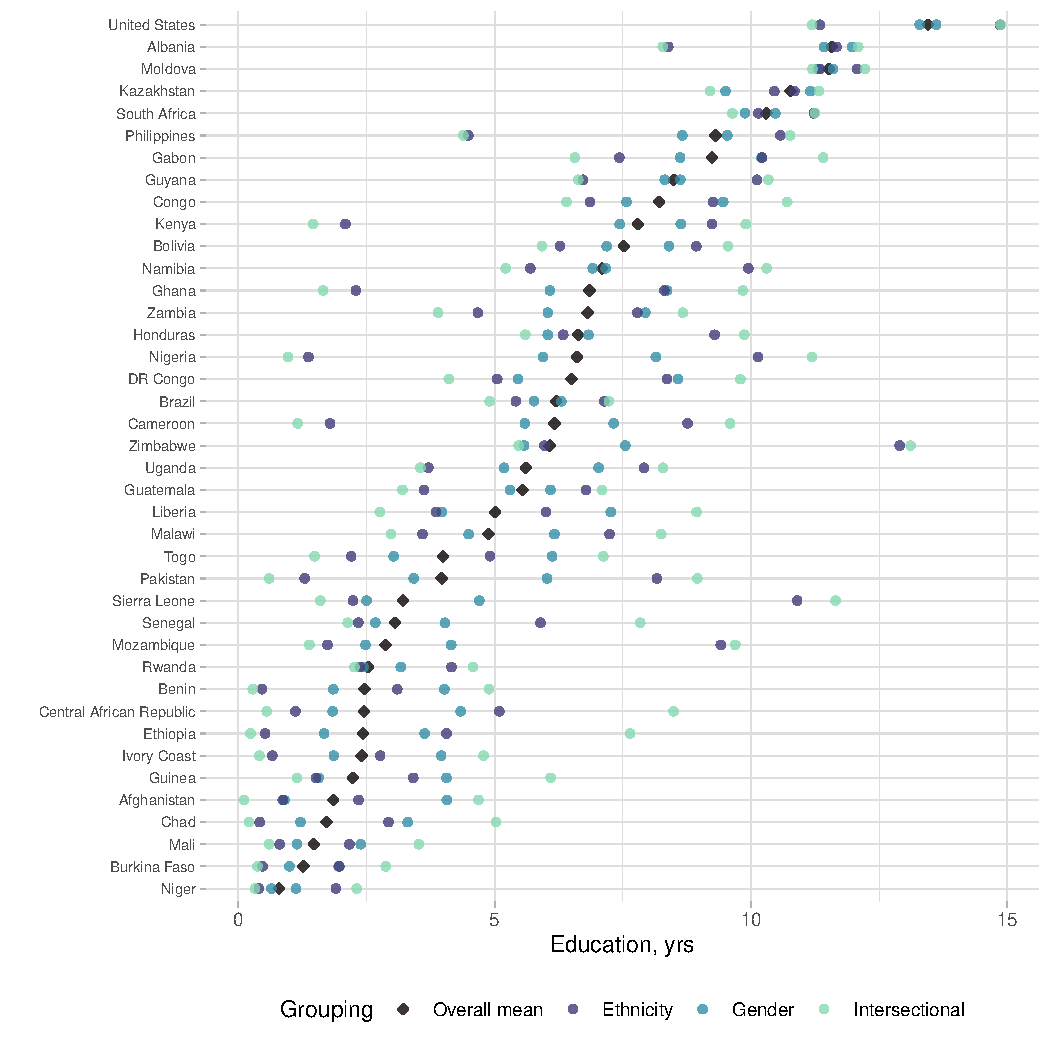
\includegraphics{latex/figures/mean-educ.pdf} \caption[Average years in education by group]{Average years in education by group}\label{fig:mean-educ}
\floatfoot{\textit{Notes:} 
Pooled data from 40 countries; $n=$2,689,279 individuals older than 25 years and younger than the birth cohort of 1920. Estimates to the right of the overall mean represent the average education of the group with the highest education. Means are calculated using DHS sample weights. Sources: DHS 1992-2019 and US CPS 2019.
} \end{figure}

\clearpage

\hypertarget{robustness-checks-with-the-theil-index}{%
\section{Robustness Checks}\label{robustness-checks-with-the-theil-index}}
\setcounter{table}{0}
\renewcommand{\thetable}{\thesection\arabic{table}}

Alternatively to the inequality ratio \(IR\) we can use a variant of the Theil Index, which is a special case of the General Entropy measures, as follows:

\[
T(G) = \frac{1}{J}\sum_{j=1}^{J}\frac{s_j}{\mu_s}arsinh(\frac{s_j}{\mu_s}),
\]

where \(s_j\) denotes the group averages, as previously defined for \(IR\), \(J\) denotes the numbers of groups and \(\mu\) the unweighted mean of all \(s_j\). Instead of the natural logarithm, as is normally used for the Theil Index, we use an inverse hyperbolic sine transformation (\(arsinh\)). It has the advantage of being defined for zero values, which is a problem that we would inevitably run into with education data from low- and middle-income countries.

Repeating the regressions shown in Table \ref{tab:ratios}, but with inequality measured by the Theil Index instead of the inequality ratio leads to the results reported in Table \ref{tab:theil}. The results remain fairly comparable.

\begin{table}

\caption{OLS regression of between-group Theil indices of education inequality\label{tab:theil}}
\centering
\begin{tblr}[         %% tabularray outer open
]                     %% tabularray outer close
{                     %% tabularray inner open
colspec={Q[]Q[]Q[]Q[]},
cell{1}{2}={c=3,}{halign=c,},
column{1}={halign=l,},
column{2}={halign=c,},
column{3}={halign=c,},
column{4}={halign=c,},
hline{21}={1,2,3,4}{solid, 0.05em, black},
}                     %% tabularray inner close
\toprule
& Group Theil Index &  &  \\ \cmidrule[lr]{2-4}
& (A) & (B) & (C) \\ \midrule %% TinyTableHeader
Mean education (yrs)$^a$ & -0.02245*** &            &            \\
& (0.00352)   &            &            \\
No. of ethnic groups     &             & 0.00296    &            \\
&             & (0.00439)  &            \\
Sample size$^b$          &             & -0.00011*  &            \\
&             & (0.00006)  &            \\
Group size lowest        &             &            & -0.00001*  \\
&             &            & (0.00000)  \\
Group size highest       &             &            & 0.00000    \\
&             &            & (0.00001)  \\
Africa                   & -0.02086    & 0.03890    & 0.05458    \\
& (0.02329)   & (0.04250)  & (0.03524)  \\
Cohort 1970-1979$^c$     & -0.00260    & -0.01576   & -0.01250   \\
& (0.00796)   & (0.01020)  & (0.01128)  \\
Cohort 1980-$^c$         & 0.00106     & -0.02475*  & -0.01974   \\
& (0.00965)   & (0.01266)  & (0.01356)  \\
(Intercept)              & 1.12170***  & 0.94132*** & 0.95245*** \\
& (0.03680)   & (0.02742)  & (0.03487)  \\
Adj. R2                  & 0.555       & 0.061      & 0.055      \\
Num.Obs                  & 105         & 105        & 105        \\
\bottomrule
\end{tblr}

\floatfoot{\textit{Notes:} Aggregated country-cohort bracket level data from 40 countries; n=2'689'279 individuals 25 years and older, and born after 1920; cluster-robust standard errors on the country-level in parentheses; Sign. codes: $^*p<10\%$, $^{**}p<5\%$, $^{***}p<1\%$. \\
$^a$~Within-country-cohort weighted mean years of education with DHS sampling weights;\\
$^b$~Within-country-cohort (individual) Gini index takes on a value between 0 and 1;
$^c$~Corresponds to country-cohort sample size in units of 1000;\\
$^d$~Ref: Cohort -1969.}
\end{table}
\FloatBarrier

\end{appendices}
\end{document}
